%% This is file `elsarticle-template-2-harv.tex',
%%
%% Copyright 2009 Elsevier Ltd
%%
%% This file is part of the 'Elsarticle Bundle'.
%% ---------------------------------------------
%%
%% It may be distributed under the conditions of the LaTeX Project Public
%% License, either version 1.2 of this license or (at your option) any
%% later version.  The latest version of this license is in
%%    http://www.latex-project.org/lppl.txt
%% and version 1.2 or later is part of all distributions of LaTeX
%% version 1999/12/01 or later.
%%
%% The list of all files belonging to the 'Elsarticle Bundle' is
%% given in the file `manifest.txt'.
%%
%% Template article for Elsevier's document class `elsarticle'
%% with harvard style bibliographic references
%%
%% $Id: elsarticle-template-2-harv.tex 155 2009-10-08 05:35:05Z rishi $
%% $URL: http://lenova.river-valley.com/svn/elsbst/trunk/elsarticle-template-2-harv.tex $
%%
\documentclass[authoryear,preprint,review,12pt]{elsarticle}

%% Use the option review to obtain double line spacing
%% \documentclass[authoryear,preprint,review,12pt]{elsarticle}

%% Use the options 1p,twocolumn; 3p; 3p,twocolumn; 5p; or 5p,twocolumn
%% for a journal layout:
%% \documentclass[final,authoryear,1p,times]{elsarticle}
%% \documentclass[final,authoryear,1p,times,twocolumn]{elsarticle}
%% \documentclass[final,authoryear,3p,times]{elsarticle}
%% \documentclass[final,authoryear,3p,times,twocolumn]{elsarticle}
%% \documentclass[final,authoryear,5p,times]{elsarticle}
%% \documentclass[final,authoryear,5p,times,twocolumn]{elsarticle}

%% if you use PostScript figures in your article
%% use the graphics package for simple commands
%% \usepackage{graphics}
%% or use the graphicx package for more complicated commands
%% \usepackage{graphicx}
%% or use the epsfig package if you prefer to use the old commands
%% \usepackage{epsfig}

%% The amssymb package provides various useful mathematical symbols
\usepackage{amssymb,amstext}
%% The amsthm package provides extended theorem environments
%% \usepackage{amsthm}

%% The lineno packages adds line numbers. Start line numbering with
%% \begin{linenumbers}, end it with \end{linenumbers}. Or switch it on
%% for the whole article with \linenumbers after \end{frontmatter}.
\usepackage{lineno}

%% natbib.sty is loaded by default. However, natbib options can be
%% provided with \biboptions{...} command. Following options are
%% valid:

%%   round  -  round parentheses are used (default)
%%   square -  square brackets are used   [option]
%%   curly  -  curly braces are used      {option}
%%   angle  -  angle brackets are used    <option>
%%   semicolon  -  multiple citations separated by semi-colon (default)
%%   colon  - same as semicolon, an earlier confusion
%%   comma  -  separated by comma
%%   authoryear - selects author-year citations (default)
%%   numbers-  selects numerical citations
%%   super  -  numerical citations as superscripts
%%   sort   -  sorts multiple citations according to order in ref. list
%%   sort&compress   -  like sort, but also compresses numerical citations
%%   compress - compresses without sorting
%%   longnamesfirst  -  makes first citation full author list
%%
%% \biboptions{longnamesfirst,comma}

\biboptions{numbers,square}

%Sik´s packages load.
\usepackage[nolist]{acronym}
\usepackage{tikz,xifthen}
\usepackage{epsf,graphicx,subfig}
\usepackage{colortbl}
\usepackage{xcolor}
\usepackage{scalefnt,lmodern}
\usepackage{booktabs, multicol, multirow}
%\usepackage{geometry}
\usepackage{pdflscape}
\usetikzlibrary{arrows,calc,positioning,backgrounds,snakes,decorations.text,decorations.markings,shapes,patterns}

%\usepackage[backend=natbib]{biblatex}
%\addbibresource{bibliografiaNew.bib}

\journal{Medical Image Analysis}
\newcommand*{\ch}{\checkmark}

\begin{document}

\definecolor{autoGuided}{rgb}{ 0.3765    0.7294    0.9412}
\newcommand{\autoGuidedColor}{(light-Blue)}
\definecolor{fullyAuto}{rgb}{ 0.0941    0.3843    0.6627}
\newcommand{\fullyAutoColor}{(dark-blue)}
\definecolor{semiAuto}{rgb}{ 0.0784    0.5059    0.1686}
\newcommand{\semiAutoColor}{(light-green)}
\definecolor{fullyGuided}{rgb}{ 0.4275    0.6902    0.3176}
\newcommand{\fullyGuidedColor}{(dark-green)}

\begin{frontmatter}
 

%% Title, authors and addresses

%% use the tnoteref command within \title for footnotes;
%% use the tnotetext command for the associated footnote;
%% use the fnref command within \author or \address for footnotes;
%% use the fntext command for the associated footnote;
%% use the corref command within \author for corresponding author footnotes;
%% use the cortext command for the associated footnote;
%% use the ead command for the email address,
%% and the form \ead[url] for the home page:
%%
%% \title{Title\tnoteref{label1}}
%% \tnotetext[label1]{}
%% \author{Name\corref{cor1}\fnref{label2}}
%% \ead{email address}
%% \ead[url]{home page}
%% \fntext[label2]{}
%% \cortext[cor1]{}
%% \address{Address\fnref{label3}}
%% \fntext[label3]{}

\title{%\LARGE \bf
%Unfinished Survey of an unbounded topic related to Breast Ultrasound images
Segmentation of breast lesions in Ultrasound images: A survey
}
\author[udg,ub]{Joan Massich}
\ead{jmassich@eia.udg.edu}
\author[udg]{Joan Mart\'{i}}
\author[ub]{Fabrice Meriaudeau}


%% use optional labels to link authors explicitly to addresses:
%% \author[label1,label2]{<author name>}
%% \address[label1]{<address>}
%% \address[label2]{<address>}

\address[udg]{Computer Vision and Robotics Group, Universitat de Girona, Campus Montilivi, Edifici PIV, s/n, 17071 Girona, Spain}
\address[ub]{Le2i-UMR CNRS 6306, Université de Bourgogne, 12 rue de la Fonderie, 712000 Le Creusot, France}

\begin{abstract}
%% Text of abstract
%Breast cancer has huge impact since it place as the leading cause of cancer death among female population. 
%Medical imaging is key for breast cancer mortality reduction, and it can increase the success of treatment,
%contributing to its early detection through screening, diagnosis, image-guided
%biopsy, treatment follow-up and suchlike procedures. Ultrasound imaging has grown into an essential tool to detect and analyze breast abnormalities. It is accepted that when US images, the most discriminative signs for diagnose are subject the lesion delimitation. Therefore the importance to develop segmentation procedures to properly delineate lesions in breast US images in order to improve computer-aided diagnosis (CAD) systems. 
%This paper reviews the approaches used for segmenting breast lesions in US images.
%The performance evaluation of segmentations is investigated as well.


Breast cancer still has huge impact due to its place as the leading cause of cancer death among female population. However, medical imaging is a key for breast cancer mortality reduction, since it can increase the success of treatment contributing to its early detection through screening, diagnosis, image-guided biopsy, treatment follow-up and suchlike procedures. Recently, \ac{us} imaging has grown into an essential tool to detect and analyze breast abnormalities, specially those present in very dense tissue. It is accepted that when dealing with \ac{us} images, the most discriminative signs for diagnose are subject to the lesion delimitation. Therefore, the importance to develop segmentation procedures to properly delineate lesions in breast \ac{us} images in order to improve \ac{cad} systems. This paper presents a taxonomy of methodologies used for segmenting breast lesions in \ac{us} images, including a review of the evaluation methodologies used to assess their performance.




\end{abstract}

\begin{keyword}
%% keywords here, in the form: keyword \sep keyword

%% MSC codes here, in the form: \MSC code \sep code
%% or \MSC[2008] code \sep code (2000 is the default)
Breast cancer; Ultrasound (US) imaging; Segmentation; Segmentation evaluation.
\end{keyword}

\end{frontmatter}

 \linenumbers

\graphicspath{{./figures/}}
\begin{acronym}[BI-RADS]
\acro{abus}[ABUS]{Automated whole Breast Ultra-Sound}
\acro{acm}[ACM]{Active Contour Model}
\acro{acr}[ACR]{American College of Radiology}
\acro{acwe}[ACWE]{Active Contour Without Edges}
\acro{adf}[ADF]{Anisotropic Diffusion Filter}
\acro{amed}[AMED]{Average Minimum Euclidian Distance}
\acro{aov}[AOV]{Area Overlap}
\acro{ard}[ARD]{Average Radial Derivative}
\acro{are}[ARE]{Average Radial Error}
\acro{birads}[BI-RADS]{Breast Imaging-Reporting and Data System}
\acro{bof}[BoF]{Bag-of-Features}
\acro{bow}[BoW]{Bag-of-Words}
\acro{bus}[BUS]{Breast Ultra-Sound}
\acro{cad}[CAD]{Computer Aided Diagnosis}
\acro{cade}[CADe]{Computer Aided Detection}
\acro{cadx}[CADx]{Computer Aided Diagnosis}
\acro{cas}[CAS]{Computer Aided Surgery}
\acro{cc}[CC]{Cranio-Caudal}
\acro{cdf}[CDF]{Cumulative Distribution Function}
\acro{crf}[CRF]{Conditional Random Field}
\acro{ct}[CT]{Computed Tomography}
\acro{cv}[CV]{Computer Vision}
\acro{dic}[DIC]{Ductal Infiltrating Carcinoma}
\acro{dicom}[DICOM]{Digital Imaging and Communications in Medicine}
\acro{dm}[DM]{Digital Mammography}
\acro{dpm}[DPM]{Deformable Part Model}
\acro{dsc}[DSC]{Dice Similarity Coefficient}
\acro{em}[EM]{Expectation Maximization}
\acro{ffdm}[FFDM]{Full-Field Digital Mammography}
\acro{fna}[FNA]{Fine Needle Aspiration}
\acro{fn}[FN]{False Negative}
\acro{fnr}[FNR]{False-Negative Ratio}
\acro{fp}[FP]{False Positive}
\acro{fpr2}[FPR]{False-Positive Ratio}
\acro{fpr}[FPR']{False-Positive Ratio'}
\acro{gc}[GC]{Graph-Cut}
\acro{gcs}[GCS]{Gaussian Constraining Segmentation}
\acro{glcm}[GLCM]{Gray-Level Co-occurrence Matrix}
\acro{gpb}[gPb]{Global Probability Boundary}
\acro{grasp}[GRASP]{Greedy Randomized Adaptive Search Procedure}
\acro{gt}[GT]{Ground Truth}
\acro{gvf}[GVF]{Gradient Vector Flow}
\acro{hd}[HD]{Hausdorff Distance}
\acro{hgte}[HGTE]{Hidden Ground Truth Estimation}
\acro{hgt}[HGT]{Hidden Ground Truth}
\acro{hog}[HOG]{Histogram of Gradients}
\acro{icm}[ICM]{Iterated Conditional Modes}
\acro{idc}[IDC]{Intra-Ductal Carcinoma}
\acro{iid}[IID]{Independent and Identically Distributed}
\acro{ilc}[ILC]{Infiltrating Lobular Carcinoma}
\acro{itg}[ITG]{Intensity Texture and Geometric}
\acro{jsc}[JSC]{Jaccard Similarity Coefficient}
\acro{lbp}[LBP]{Local Binary Pattern}
\acro{loo}[LOOCV]{Leave-One-Out Cross-Validation} 
\acro{mad}[MAD]{Median Absolute Deviation}
\acro{map}[MAP]{Maximum A Posteriori}
\acro{mcde}[MCDE]{Modified Curvature Diffusion Equation}
\acro{md}[MD]{Minimum Distance}
\acro{ml}[ML]{Machine Learning}
\acro{mlo}[MLO]{Medio-Lateral Oblique}
\acro{mra}[MRA]{Multi Resolution Analysis}
\acro{mrf}[MRF]{Markov Random Field}
\acro{mri}[MRI]{Magnetic Resonance Image}
\acro{nc}[NC]{Normalized Cuts}
\acro{npv}[NPV]{Negative Predictive Value}
\acro{nrv}[NRV]{Normalized Residual Value}
\acro{of}[OF]{Overlap Fraction}
\acro{pca}[PCA]{Principal Component Analysis}
\acro{pde}[PDE]{Partial Differential Equation}
\acro{pdf}[PDF]{Probability Density Function}
\acro{pd}[PD]{Proportional Distance}
\acro{pet}[PET]{Position Emission Tomography}
\acroplural{roi}[ROIs]{ Regions Of Interest}
\acro{ppv}[PPV]{Positive Predictive Value}
\acro{pr}[PR]{Pattern Recognition}
\acro{qc}[QC]{Quadratic-Chi}
\acro{qs}[QS]{Quick-Shift}
\acro{rbf}[RBF]{Radial Basis Function}
\acro{rf}[RF]{Random Forest}
\acro{rgi}[RGI]{Radial Gradien Index}
\acro{rgi}[RGI]{Radial Gradient Index}
\acro{rg}[RG]{Region Growing}
\acro{roi}[ROI]{Region Of Interest}
\acro{sa}[SA]{Simulated Annealing}
\acro{sift}[SIFT]{Self-Invariant Feature Transform}
\acro{si}[SI]{Similarity Index}
\acro{slic}[SLIC]{Simple Linear Iterative Clustering}
\acro{snr}[SNR]{Signal to Noise Ratio}
\acro{som}[SOM]{Self Organizing Map}
\acro{staple}[STAPLE]{Simultaneous Truth and Performance Level Estimation}
\acro{svm}[SVM]{Support Vector Machine}
\acro{tnr}[TNR]{True-Negative Ratio}
\acro{tn}[TN]{True Negative}
\acro{tpr}[TPR]{True-Positive Ratio}
\acro{tp}[TP]{True Positive}
\acro{us}[US]{Ultra-Sound}
\end{acronym}

Breast cancer is the second most common cancer (1.4 million cases per year, 10.9\% of  diagnosed cancers) after lung cancer, followed by colorectal, stomach, prostate and liver cancers~\cite{Ferlay2010}. 
In terms of mortality, breast cancer is the fifth most common cause of cancer death. However, it places as the leading cause of cancer death among females both in western countries and in economically developing countries~\cite{cancerStatistics2011}.

Medical imaging plays an important role in breast cancer mortality reduction, contributing to its early detection through screening, diagnosis, image-guided biopsy, treatment follow-up and suchlike procedures~\cite{smith2003american}.
Although \ac{dm} remains the reference imaging modality, \ac{us} imaging has proven to be a successful adjunct image modality for breast cancer screening~\cite{smith2003american,berg2004diagnostic}, specially as a consequence of the discriminative capabilities that \ac{us} offers for differentiating between solid lesions that are benign or malignant~\cite{Stavros:1995p12392} so that the amount of unnecessary biopsies, which is estimated to be between $65\sim85\%$ of the prescribed biopsies~\cite{yuan2010multimodality}, can be reduced~\cite{ciatto1994contribution} in replacing them by short-term \ac{us} screening follow-up~\cite{gordon1995malignant}.

Regardless of the clinical utility of the \ac{us} images, such image modality suffers from different inconveniences due to strong noise natural of \ac{us} imaging  and the presence of strong \ac{us} artifacts, both degrading the overall image quality~\cite{Ensminger:2008p6920} which compromise the performance of the radiologists. Radiologists infer health state of the patients based on visual inspection of images which by means of some screening technique (e.g.~\ac{us}) depict physical properties of the screened body. The radiologic diagnosis error rates are similar to those found in any other tasks requiring human visual inspection, and such errors, are subject to the quality of the images and the ability of the reader to interpret the physical properties depicted on them \cite{manning2005perception}.

Therefore the major goals of medical imaging researchers in general, and also in particular for breast lesion assessment using \ac{us} data, have been to provide better instrumentation for improving the image quality, as well as, methodologies and procedures in order to improve the interpretation of the image readings. In image interpretation unified terms for characterizing, describing and reporting the lesions have been developed~\cite{Stavros:1995p12392,mendelson2001toward,biradsus,stavros2004breast} in order to reduce diagnosis inconsistencies among readers~\cite{baker1999sonography}. Such unifying terms so called lexicons are proven to be a useful framework for the radiologists when analyzing \ac{bus} images. The \ac{ppv} and \ac{npv} which represent the percentage of properly diagnosed cases~\cite{altman1994statistics} achieved when describing lesions with these lexicon tools turned them into the standard for human reading and diagnosis based on \ac{bus} images. 

A common framework allows managing the \ac{us} imaging inconveniences such as strong noise or artifacts by allowing the comparison of double readings done by several specialized observers. The major inconvenience for double reading is the elevated time required from the radiologists. Thus, since a single observer using \ac{cad} as a second opinion has been proven to achieve comparable results~\cite{giger2008anniversary}, \ac{cad} systems are used to alleviate the time demand from the radiologists. 

\ac{cad} systems applied to aid radiologist when reading \ac{us} images of the breast take advantage of either low-level features, high-level features or both~\cite{Cheng:2009p10580}. Jalalian et al.~\cite{jalalian2012computer} reported that the majority of such hig-level features describing the lesions which bring reliable information to the systems, can be found in these lexicon tools already used by radiologists~\cite{biradsus,stavros2004breast}. However, to take advantage of these descriptors, procedures to accurately segment the lesions are needed. This need comes from the fact that when the images are read by an expert radiologist, the underlying delineation of the lesion is instantly understood.

This article reviews recent advances in breast lesion segmentation in \ac{us} data procedures which can be used for further extracting reliable high-level features for improving \ac{cad} systems applied to breast \ac{us} images.
%
%
%\ac{us} imaging has proven to be a successful adjunct image modality for breast cancer screening~\cite{smith2003american,berg2004diagnostic}, especially in view of the discriminative capabilities that \ac{us} offers for differentiating between benign or malignant solid lesions~\cite{ciatto1994contribution}. As a result, the number of unnecessary biopsies, which is estimated to be between $65\sim85\%$ of all prescribed biopsies~\cite{yuan2010multimodality}, can be reduced~\cite{ciatto1994contribution} with the added advantage of a close follow-up with sequential scans~\cite{gordon1995malignant}.
%
%%However, the noisy nature of the \ac{us} image modality and the presence of strong artifacts, both degrading the overall image quality~\cite{Ensminger:2008p6920}, raise diagnosis error rates as would happen in any other human visual inspection task~\cite{manning2005perception}. Therefore, uniform terms in order to reduce diagnosis inconsistencies among readers~\cite{baker1999sonography} characterizing, describing and reporting the lesions have been developed~\cite{Stavros:1995p12392,mendelson2001toward,biradsus,stavros2004breast} so that double readings can be performed and a more accurate diagnosis achieved. The main inconvenience of double readings is cost, justifying the use of \ac{cad} systems, which have also proven to improve diagnosis accuracy~\cite{giger2008anniversary}. 
%
%\ac{bus} \ac{cadx}, as mentioned earlier, can take advantage of either low-level features, high-level features or both~\cite{Cheng:2009p10580}. However, in order to take advantage of high-level features or descriptors similar to the lexicon descriptors proposed in~\cite{biradsus,stavros2004breast}, an accurate segmentation is needed (see section~\ref{lexicon}). 

\section[The role of segmentation in breast US CAD system]{The role of segmentation within a Breast ultrasound Computer Aided Diagnosis (CAD) system}\sectionmark{The role of segmentation in CAD }\label{section:userInteraction}

Segmentation is a fundamental procedure for a \ac{cad} system. Figure~\ref{fig:cadseg} illustrates the idea that procedures for segmentating breast lesions in \ac{us} data can be found within a \ac{cad} system workflow as part of \ac{cade}, as part of \ac{cadx} or as a stand alone step using detection information and providing further information that can be used for conducting a diagnosis. 

%The segmentation within a workflow of the \ac{cad} system consists of a block between detection and diagnosis which can be integrated to any of the two or neither of them in the sense that there exist \ac{cade} systems providing an accurate segmentation as an output  or \ac{cadx} that generates segmentations from user inputs in order to extract accurate features to drive the diagnosis. Figure~\ref{fig:cadseg} graphically represents such idea.

\begin{figure}[htbp]
\centering
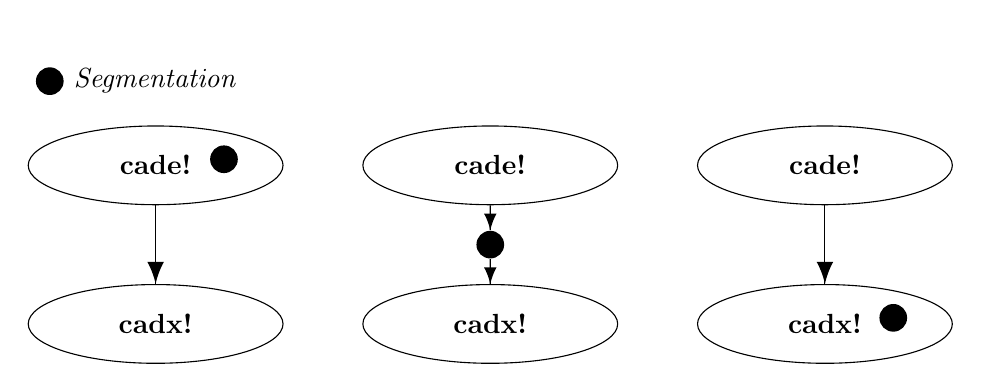
\begin{tikzpicture}[auto, >=latex]
		 
	 \def\scale{2}
	 \def\segDotDistance{-8pt}
	 \tikzset{dot/.style={circle,fill=black,inner sep=0mm,minimum size=10pt}}
	 \tikzset{elip/.style={draw,ellipse, minimum width={\scale*1.618cm},minimum height={\scale*.5cm} }}
	  
	 
	 
	 \draw node [elip] (cade1) {\acs{cade}}
	 	   node [elip,right= of cade1] (cade2) {\acs{cade}}
		   node [elip,right= of cade2] (cade3) {\acs{cade}}
		  
		   node [elip, below= of cade1] (cadx1) {\acs{cadx}}
	 	   node [elip, right= of cadx1] (cadx2) {\acs{cadx}}
		   node [elip, right= of cadx2] (cadx3) {\acs{cadx}} 

		   node [ above= of cade1] (aux) {}
		   ($(cade1.north) !.5! (aux)$) node (segName) {\emph{Segmentation}}
		   ;

	\draw ($(cade1.north east)$) ++({\segDotDistance},{\segDotDistance}) node [dot] {}
		  ($(cadx3.north east)$) ++({\segDotDistance},{\segDotDistance}) node [dot] {}
		  ($(segName.west)$) node [dot, left]{}
		  ($ (cade2) !.5! (cadx2) $) node [dot] (d){}
	;

	 \draw [ decoration={markings,mark=at position 1 with {\arrow[scale=2]{>}}},  postaction={decorate}] 	(cade1) -- (cadx1) ;
	 \draw  [ decoration={markings,mark=at position 1 with {\arrow[scale=1.5]{>}}},  postaction={decorate}]  	(cade2) -- (d) ;
	 \draw  [ decoration={markings,mark=at position 1 with {\arrow[scale=1.5]{>}}},  postaction={decorate}] 	(d) -- (cadx2);
	 \draw  [ decoration={markings,mark=at position 1 with {\arrow[scale=2]{>}}},  postaction={decorate}]  	(cade3) -- (cadx3) ;	 
		   

\end{tikzpicture}
\caption[Role of segmentation procedures within \ac{cad} systems.]{Illustrative idea of the role of segmentation within a \ac{cad} framework showing that it can either be a separate process between a \ac{cade} and a \ac{cadx} or it can belong to any of the two \ac{cad} typologies: \ac{cade}, \ac{cadx} }
\label{fig:cadseg}
\end{figure}


Segmentation procedures integrated within \ac{cad} systems can either be manual, interactive or automatic depending on the amount of effort or data supplied by the user. 
\ac{cadx} systems needing high-level descriptors supplied by a user or a non-aided manual delineation also fall into the manual category and therefore, are not extensively reviewed. As an example of this category, we cite the work presented by Hong et al.~\cite{Hong:2005p14207}, which describes a system working on \ac{birads} descriptors supplied by an expert based on the reading of images. 

%Notice that for manual it is understood non aided delineations or \ac{cadx} systems that need of high-level descriptors supplied by a user. As example, the work presented by Hong et al.~\cite{Hong:2005p14207} falls into such category since the system works on \ac{birads} descriptors supplied by an expert based on the reading of images. 

Figure~\ref{fig:segmentationInteractivityTable} compiles methodologies of interest and categorizes them according to the following groups and subgroups:

\begin{description}
\item[Interactive Segmentation:] methodologies requiring any kind of user interaction to drive the segmentation.
	\begin{itemize}
		\item \emph{Fully-Guided} are those methodologies where the user is asked to accompany the method through the desired delineation.
		\item \emph{Semi-Automatic} are those methodologies where the segmentation is conditioned by the user by means of labeling the regions instead of the delineation path.
	\end{itemize} 
\item[Automatic Segmentation:] methodologies with no user interaction.
	\begin{itemize}
	\item \emph{Auto-Guided} are an evolution of Semi-Automatic methodologies so that user interaction has been substituted by an automatic procedure (usually as an automatic initialization of the original Semi-Automatic procedure). 
	
	\item \emph{Fully-Automatic} are ad-hoc automatic procedures designed in such a manner that no user interaction can be incorporated.
	\end{itemize} 
\end{description}

%\begin{table}
%\label{fig:segmentationInteractivityTable}
%\caption
%\begin{tabular}{r l l}
%
%  group & subgroup & method highlights\\
%  \hline  \hline
%  interactive & fully guided & JetStream \cite{Angelova:2010p14355} \\
%  
%  & semi-Automatic & \acs{gcs}, \acs{ard} \cite{Horsch:2001p6028} \\
%  & & \acs{gcs}\cite{massich2010lesion} \\
%  & & \acs{gcs}, watershed \cite{Gomez:2010p14339} \\
%  & & \acs{map}-\acs{mrf}, \acs{em} \cite{Xiao:2002p5639,gerard2013} \\
%  & & Grabcut, watershed \cite{chiang2010cell}\\
%  & & \acs{acm}, gradient LevelSet, geodesic snake  \cite{AlemanFlores:2007p14310} \\
%  & & snake \cite{Cui:2009p14325}\\
%  & & GVF-LevelSets \cite{Gao:2012p14336} \\
%  \hline
%  automatic & auto-guided & \acs{gcs}, \acs{rgi} \cite{Drukker:2002p10442} \\
%  & & \acs{map},texture, \acs{gcs} \cite{massich2010lesion,massich2011seed,massich2012seed} \\
%  & & \acs{map}, texture, \acs{rg}, snake \cite{Madabhushi:2003p6036} \\
%  & & Th\cite{otsu1975threshold}, application criteria, snake \cite{Huang:2007p6100} \\
%  & & \acs{ml} detection, \acs{ml} segmentation \cite{Zhang:2010p14317} \\
%  & & \acs{ml} detection, \acs{ml} segmentation \cite{Jiang:2012p14354} \\
%  & & Th\cite{otsu1975threshold}, application criteria\cite{Shan:2008p10923} for cropping, \acs{ml} segmentation  
%\cite{Shan:2012p14347} \\
%
%  & fullyAutomatic & watershed, texture merging, GVF-snake \cite{Huang:2005p11636} \\
%  & & unsupervised \ac{ml}, graph representation, merging, snake \cite{Huang:2012p14313} \\
%  & & \acs{nc}, graph representaiton, merging, morphology  \cite{Liu:2005p14341} \\
%  & & Objective function, \acs{gc}, \acs{dpm}\cite{felzenszwalb2010object},\acs{glcm} \cite{hao2012combining} \\
%  & & Watershed  \cite{Huang:2004p2092} \\
%  & & \ac{ml} \cite{Liu:2010p12036} \\
%  & & Model driven LevelSet \cite{Liu:2010p14328} \\
%  & & Inpainting \cite{Yeh:2009p11985} \\
%  \hline
%\end{tabular}
%\end{table}


%\begin{tiny}
%•
%\end{tiny}
\begin{figure}
     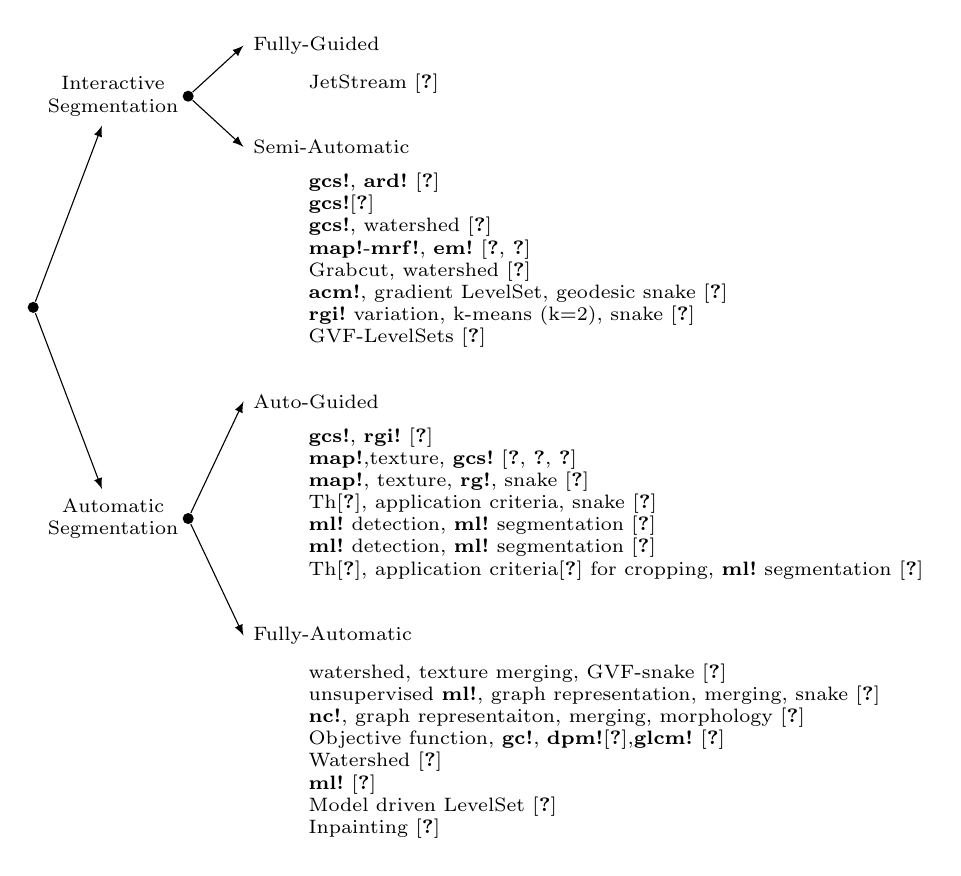
\begin{tikzpicture}[auto, >=latex, node distance=1pt,font=\scriptsize]

	\def\fullyGuidedMethods{JetStream \cite{Angelova:2010p14355}}
    \def\semiAutoMethods{\acs{gcs}, \acs{ard} \cite{Horsch:2001p6028} \\ \acs{gcs}\cite{massich2010lesion} \\\acs{gcs}, watershed \cite{Gomez:2010p14339} \\\acs{map}-\acs{mrf}, \acs{em} \cite{Xiao:2002p5639,gerard2013} \\ Grabcut, watershed \cite{chiang2010cell}\\ \acs{acm}, gradient LevelSet, geodesic snake  \cite{AlemanFlores:2007p14310} \\
												\acs{rgi} variation, k-means (k=2), snake \cite{Cui:2009p14325}\\
												GVF-LevelSets \cite{Gao:2012p14336}}
	  \def\autoGuidedMethods{	\acs{gcs}, \acs{rgi} \cite{Drukker:2002p10442} \\
													\acs{map},texture, \acs{gcs} \cite{massich2010lesion,massich2011seed,massich2012seed} \\
													\acs{map}, texture, \acs{rg}, snake \cite{Madabhushi:2003p6036} \\
													Th\cite{otsu1975threshold}, application criteria, snake \cite{Huang:2007p6100} \\
													\acs{ml} detection, \acs{ml} segmentation \cite{Zhang:2010p14317} \\
													\acs{ml} detection, \acs{ml} segmentation \cite{Jiang:2012p14354} \\
													Th\cite{otsu1975threshold}, application criteria\cite{Shan:2008p10923} for cropping, \acs{ml} segmentation \cite{Shan:2012p14347}}
	\def\fullyAutoMethods{watershed, texture merging, GVF-snake \cite{Huang:2005p11636} \\
unsupervised \acs{ml}, graph representation, merging, snake \cite{Huang:2012p14313} \\
\acs{nc}, graph representaiton, merging, morphology  \cite{Liu:2005p14341} \\
Objective function, \acs{gc}, \acs{dpm}\cite{felzenszwalb2010object},\acs{glcm} \cite{hao2012combining} \\
Watershed  \cite{Huang:2004p2092} \\
\acs{ml} \cite{Liu:2010p12036} \\
Model driven LevelSet \cite{Liu:2010p14328} \\
Inpainting \cite{Yeh:2009p11985}			}						

%% Draw the groups and the lists
\def\listIndent{20pt}
\def\listNameSpace{-10pt}
\draw (0,0) node [right] (fullyguided) {Fully-Guided}
		   ($(fullyguided.south west)$) ++({\listIndent},0) node [anchor=north west,align=left] (fullyguided_) {\fullyGuidedMethods}
		   ($(fullyguided_.south west)$) ++({-1*\listIndent},\listNameSpace) node [anchor=north west] (semiAuto){Semi-Automatic}
		   ($(semiAuto.south west)$) ++({\listIndent},0) node [anchor=north west,align=left] (semiAuto_) {\semiAutoMethods}
		   ($(semiAuto_.south west)$) ++({-1*\listIndent},\listNameSpace) node [anchor=north west] (autoGuide) {Auto-Guided}
		   ($(autoGuide.south west)$) ++({\listIndent},0) node [anchor=north west,align=left] (autoGuided_) {\autoGuidedMethods}
		   ($(autoGuided_.south west)$) ++({-1*\listIndent},\listNameSpace) node [anchor=north west] (fullyAuto){Fully-Automatic}
		   ($(fullyAuto.south west)$) ++({\listIndent},0) node [anchor=north west,align=left] (autoGuide_) {\fullyAutoMethods}
		   ;
		   
%% Draw the relations
 \tikzset{pt/.style={circle,fill=#1,inner sep=0mm,minimum size=4pt}}
 \draw ($ (fullyguided.west) !.5! (semiAuto.west) $) ++({-1*\listIndent},0) node [pt=black] (guideDot) {} node [left,align=center] (interactiveName) {Interactive \\ Segmentation };
 \draw ($ (autoGuide.west) !.5! (fullyAuto.west) $) ++({-1*\listIndent},0) node [pt=black] (autoDot) {} node [left,align=center] (automaticName) {Automatic \\ Segmentation }; 
 \draw ($ (guideDot) !.5! (autoDot) $) ++({-2.8*\listIndent},0) node [pt=black] (ini) {};   
  
 \draw [->] 	(guideDot) -- (fullyguided.west);
 \draw [->]	(guideDot) -- (semiAuto.west);
 \draw [->] 	(autoDot) -- (autoGuide.west);
 \draw [->]	(autoDot) -- (fullyAuto.west);
 \draw [->] (ini) -- (interactiveName);
 \draw [->]	(ini) -- (automaticName);
% \draw [decoration={text along path,  text={Automatic},text align={center}},decorate] 	(ini) -- (autoDot);
  
     \end{tikzpicture}
 \caption[List of breast lesion segmentation methodologies and their highlights.]{List of breast lesion segmentation methodologies and their highlights. The methodologies are groped in two categories: interactive and automatic; with  four subcategories: Fully-Guided, Semi-Automatic, Auto-Guided and Fully-Automatic.} \label{fig:segmentationInteractivityTable}
    
  \end{figure}

\subsection{Interactive Segmentation}   
While fully automatic segmentation still remains unsolved, it is obvious that manual delineations are unacceptably laborious and the results suffer from huge inter- and intra-user variability, which reveals its inherent inaccuracy.
Thus, interactive segmentation is rising as a popular alternative alleviating the inherent problems in fully automatic or manual segmentation by taking advantage of the user to assist the segmentation procedure. Interactive methodologies are mainly designed as general purpose techniques since the segmentation is controlled by a skilled user who supplies the knowledge regarding the application domain. 
Depending on the typology of information the user provides the system in order to govern the segmentation, two distinct strategies can be differentiated: \emph{fully-guided} and \emph{semi-automatic}. 

For a fully-guided strategy, the user indicates the boundary of the desired segmentation and accompanies the procedure along the whole path. Some successful general purpose techniques that require this kind of user interaction, and just to name a couple, are: \emph{intelligent-scissors}~\cite{mortensen1998interactive}, or \emph{Jetstream} segmentation~\cite{perez2001jetstream}, both deriving from the \emph{live-wire} technique~\cite{falcao1998user}, which requires the user to indicate roughly the path of the desired boundary and the segmentation procedure automatically adjusts to the underlying desired partition in an interactive manner. 

For a semi-automatic strategy, the user constrains or initializes the segmentation procedure by indicating parts or elements belonging to each object to be segmented (i.e. foreground/background).  The segmentation procedure generates the final delineation from this information. Two popular general purpose interactive segmentation techniques falling in this category are: \emph{lazy snapping}~\cite{li2004lazy} and \emph{grabcut}~\cite{rother2004grabcut} both based on the work proposed by Boykov and Jolly~\cite{boykov2001interactive} which takes advantage of \ac{gc} and a naive indication of the elements present within the image to find a proper delineation of the object of interest.

Although interactive segmentation procedures are designed in a general manner, due to the difficulties present in \ac{us} images, some interactive segmentation procedures especially designed for delineating breast lesions in \ac{us} data have been developed. The remainder of this section compiles these procedures in terms of the aforementioned fully-guided and semi-automatic terms.

%The user either  supplies information indicating the desired boundary leading to a \emph{fully-guided} procedure, or otherwise, the user constraints  or initializes the segmentation procedure by indicating parts or elements belonging to each object to be segmented (i.e. foreground/background) leading to a \emph{semi-automatic} segmentation procedure. As example of general purpose interactive segmentation, and just to name a few, intelligent-scissors~\cite{mortensen1998interactive}, or, Jetstream segmentation~\cite{perez2001jetstream} both deriving from live-wire~\cite{falcao1998user} require the user to indicate rough path of the desired boundary and such approaches adjust to the underlying desired partition. Techniques such as lazy snapping~\cite{li2004lazy} or grabcut~\cite{rother2004grabcut} are based on the work proposed by Boykov and Jolly~\cite{boykov2001interactive} which takes advantage of graph cuts and a naive indication of the elements to find a proper snap of the object of interest.

%(in those particular cases) 
%
%order to split the image in foreground and background; or intelligent-sissors~\cite{mortensen1998interactive}), or, Jetstream segmentation~\cite{perez2001jetstream} both derived from live-wire~\cite{falcao1998user} just to name a few. 
%
%Such techniques take advantage of the user which assist the segmentation by suppling either information of the objects by indicating regions of interest, or by suppling information indicating the desired boundary. Based on those behaviors, interactive segmentation techniques can be roughly split into two class depending on the typology of information required to the user, here called fully-guided and semi-automatic. Where the fully-guided strategies~\cite{falcao1998user,mortensen1998interactive,perez2001jetstream} demand to the indicate the boundary between regions of interest and semi-automatic procedures demand to the user to indicate which region belongs to each object~\cite{boykov2001interactive}.

\subsubsection{Fully-guided interactive segmentation applied to Breast Ultrasound images}

Due to the quantity of knowledge extracted from the user when segmenting with a fully-guided interactive procedure, it is rare to find a fully-guided segmentation designed for a particular application. However, Angelova and Mihaylova~\cite{Angelova:2010p14355,Angelova:2009p14781} implemented a jetstream~\cite{perez2001jetstream} especially designed to be applied to segment breast lesions in \ac{us} data images. 

It can be argued that their proposal is not a fully-guided procedure as the authors have limited the user interactivity since it is not allowed to condition the segmentation along the whole path. The method is initialized by four point locations indicating the center of the lesion, an inner bound, an outer bound, and a point lying within the desired boundary. These four locations drive the whole segmentation that takes advantage of intensity and position information. In this sense the methodology can be categorized as semi-automatic. However, it has been considered fully-guided since it is based on a fully-guided procedure, namely jet stream. Implementation of multiple reinitialization of the boundary location in order to achieve fully-guidance is straight forward despite not being covered in the original work. 

The evaluation of the method is done in a qualitative manner using a dataset of 20 images. No quantitative results are reported. 

%Although the authors are not aware of any fully-guided procedure specifically designed for breast lesion segmentation in \ac{us} data, it does exist a variation of the jetstream, which is indeed a fully-guided segmentation procedure, specifically designed for breast lesions and \ac{us} data proposed by Angelova and Mihaylova~\cite{Angelova:2010p14355,Angelova:2009p14781}. However instead of letting the user inserting seed points along the desired contour to guide the segmentation process, the method asks for three control points and a seed laying in the contour. The method uses those four locations to drive a segmentation at once taking advantage of intensity and position information. Therefore it can be argued that~\cite{Angelova:2010p14355} falls into the semi-automatic category although is based on a fully-guided procedure. The evaluation of the method is done in a qualitative manner using a dataset of 20 images. No quantitative results are reported. 


\subsubsection{Semi-automatic segmentation applied to Breast Ultrasound images}\label{sec:semi-auto}
In this section we consider semi-automatic segmentation methods; those methods requiring the user to impose certain hard constraints like indicating that certain pixels (seeds) belong to a particular object (either lesion or background).

%Horsch et al.~
\cite{Horsch:2001p6028} propose a method using a \ac{gcs} consisting of combining a Gaussian shape totally or partially defined by the user with an intensity dependent function. The final segmentation consists of finding the contour resulting from thresholding the Gaussian constrained function that maximizes the \ac{ard} measure. The maximization is done in an exhaustive manner. The segmentation performance was tested on a 400 image dataset achieving a mean \ac{aov} of $0.73$ when compared to manual delineation by an expert radiologist.  Massich et al.~\cite{massich2010lesion} proposed a methodology inspired by \ac{gcs} with different user interactability levels that falls into the interactive and semi-automatic procedures category when manually initialized with a single click. The difference between this work and the original \ac{gcs} methodology lies in the intensity dependent function and the manner in which the final threshold is chosen since a disparity measure is minimized instead of maximizing the \ac{ard} coefficient. In this proposal, the intensity dependent function used is robust to the thresholding so that if, instead of dynamically choosing a thresholding based on the error measure or \ac{ard}, a fixed threshold (properly tuned for the dataset) is preferred, the segmentation results are consistent. Although a slightly lower performance in terms of mean is reported, $0.66$ compared to $0.73$ obtained by the original \ac{gcs} methodology, there is no difference statistically when comparing the result distribution in a common dataset~\cite{massich2010lesion}, and the methodology proposed by Massich et al. demands less user interaction. 
Another work based on \ac{gcs}~\cite{Horsch:2001p6028} is the work proposed by Gomez et al.~\cite{Gomez:2010p14339} where watershed transform is used to condition the intensity dependent function. As in the original \ac{gcs} proposal, \ac{ard} maximization is used in order to find the adequate threshold that leads to the final segmentation. Although a larger dataset should be used in order to corroborate the improvement and the fact that the multivariate Gaussian is determined by 4 points supplied by the user, a mean overlap of $0.85$ is reported using a 20 image dataset. 

In Xiao et al.~\cite{Xiao:2002p5639}, the user is required to determine different \acp{roi} placed inside and outside the lesion in order to extract the intensity distribution of both. Then, these distributions are used to drive an \ac{em} procedure over the intensity spectrum of the image incorporating a \ac{mrf} used for both smoothing the segmentation and estimating the distortion field. Although in~\cite{Xiao:2002p5639} the method is only qualitatively evaluated in a reduced set of synthetic and real data, further studies reducing the user interaction from different \acp{roi} to a single click~\cite{gerard2013} reported results using two larger datasets of 212 and 140 images obtaining an \ac{aov} of $0.508$ for the original method and $0.55$ for the less interactive proposal, and a \ac{dsc} score of $0.61$ and $0.66$ respectively. 

Other examples of semi-automatic procedures addressing segmentation of breast lesions in \ac{us} images are: the implementation of the grab-cut methodology proposed by Chiang et al.~\cite{chiang2010cell} or the various manually initialized implementations of the popular \acp{acm} technique~\cite{AlemanFlores:2007p14310,Cui:2009p14325,Gao:2012p14336}. These \ac{acm} methodologies reported really good results achieving a mean \ac{aov} of $0.883$ for the implementation presented in~\cite{AlemanFlores:2007p14310}. Within the group of methodologies using \ac{acm},  Alem{\'a}n-Flores et al.~\cite{AlemanFlores:2007p14310} connected two completely different \ac{acm} procedures in a daisy-chain manner. First, the image is simplified by applying a modified \ac{adf} that takes texture into account, using the Gabor filter responses to drive the amount of diffusion. Then, a manual seed is used to initialize a gradient regularized LevelSet method as if it were a region growing procedure growing in the simplified image. Finally, the pre-segmentation\footnote{The segmentation obtained from the first \ac{acm} procedure.} obtained is used to initialize a geodesic snake \ac{acm} that evolves using intensity information from the inner and outer parts.
In a similar way, Cui et al.~\cite{Cui:2009p14325} evolves two \acp{acm} in a daisy chain manner. However, in this case the \acp{acm} are identical, differing only in their initialization. Finally, the best solution from the two \acp{acm} is selected. A mean \ac{aov} of $0.74$ was reported on a large dataset of 488 images. Gao et al.~\cite{Gao:2012p14336} tested on a small dataset of 20 images the use of a GVF-based LevelSet \ac{acm} that also took into account the phase congruency texture~\cite{kovesi2000phase} along with the gradient information, achieving a mean \ac{aov} of $0.863$.


\subsection{Automatic Segmentation}
Although automatic segmentation of breast lesions in ultrasound images remains unsolved, huge efforts 
to obtain lesion delineations with no user interaction have been made in the last few years. In order to categorize the automatic segmentation methodologies, two distinct strategies when designing the methodologies have been adopted for classification: methodologies automatizing semi-automatic procedures so that no user interaction is required, and ad-hoc methodologies designed in a manner that no element can be substituted by user supplied information. 

The former has been named \emph{auto-guided} procedures since for this case the information supplied by the user has been substituted by an automatic methodology that guides the semi-automatic segmentation, while the latter have been identified as \emph{fully automatic} procedures.

Notice that for this work, only methodologies outputting a segmentation are reviewed. Therefore, \ac{cade} procedures that can be used to initialize a semi-automatic procedure are out of the study unless there is explicitly paired work such as in (Drukker et al.~\cite{Drukker:2002p10442} , Horsch et al.~\cite{Horsch:2001p6028}) or (Shan et al.~\cite{Shan:2008p10923}, (Shan et al.~\cite{Shan:2012p14347}). 

\subsubsection{Auto-guided Segmentation}
Listed here are segmentation methodologies that consist of automatizing semi-automatic procedures or methodologies  conceived as a two step problem: lesion detection and further segmentation of any detected lesions; methodologies that in some sense can be seen as a decoupled \ac{cade} and further segmentation. 

A clear example of this group is the work proposed by Drukker et al.~\cite{Drukker:2002p10442} where an automatic detection procedure is added to the original \ac{gcs} segmentation~\cite{Horsch:2001p6028} eliminating user interaction.

In order to properly detect the lesion to successfully delineate it using \ac{gcs}, several rough \ac{gcs} segmentations are performed in a sparse regular grid. Every position on the grid is constrained (one at a time) with a constant bivariate Gaussian function. The resulting Gaussian constrained image depending function is thresholded at several levels in order to generate a set of delineations. The \ac{rgi}\footnote{This differs from the \ac{gcs} procedure used for the final delineation since \ac{ard} index is used.} is calculated for all the delineations of every delineation set. The maximum \ac{rgi} reward of every delineation set is used to  generate a low resolution image which is thresholded to determine an approximation of the lesion's boundaries. This approximation is used to determine a seed point in order to control the final segmentation as proposed in~\cite{Horsch:2001p6028}. The method was evaluated solely as a detection in a 757 image dataset achieving a TPR of $0.87$ and a FPR of $0.76$. 

Massich et al.~\cite{massich2010lesion} also proposed a methodology based on \ac{gcs} as~\cite{Drukker:2002p10442} with several levels of user interaction contemplating the no user interaction scenario. The method consists of a 4 step procedure: seed placement procedure (\ac{cade}), a fuzzy region growing, a multivariate gaussian determination, and finally, a \ac{gcs}. The seed placement produces an initial region that is further expanded. Once expanded, the final region is used to determine a multivariate Gaussian which can have any orientation.
This is an improvement with respect to the original \ac{gcs} formulation in~\cite{Horsch:2001p6028} allowing better description of oblique lesions since, in the original work, only Gaussian functions orthogonal to the image axis were considered. Similar to the original work, this constraining Gaussian function is used to constrain an intensity dependent function that is thresholded in order to obtain the final delineation. The intensity dependent function and the manner of determining the most appropriate threshold differ in the two proposals. The method is evaluated using a dataset of 25 images with multiple \ac{gt} annotations. For evaluation purposes, the multiple annotations are combined using \ac{staple}~\cite{Warfield:2004p9614} in order to obtain the \ac{hgt}. Then the methodology is assessed in terms of area overlap with the merging of the delineations weighted by the \ac{hgt} saliency, achieving a reward coefficient of $0.64$ with no user interaction. Those results are comparable to the results achieved by~\cite{Horsch:2001p6028} since segmentations obtained from missed or wrongly detected lesions were also taken into account to produce the assessing results. Further details on the exact seed placement algorithm can be found in~\cite{massich2011seed,massich2012seed}. This seed placement is based on  a multi-feature Bayesian \ac{ml} framework to determine whether a particular pixel in the image is a lesion or not. From the learning step, a \ac{map} probability plane of the target image is obtained and thresholded with certain confidence ($0.8$ as reported in~\cite{massich2012seed}). Then the largest area is selected as the candidate region for further expansion. Due to the sparseness of the data within the feature space, \ac{iid} is assumed so that \ac{map} can be calculated from the marginals of each feature, a fact that does not always hold indicates that more complex models are needed.

Madabhushi and Metaxas~\cite{Madabhushi:2003p6036} proposed using the \emph{Stavros Criteria} \cite{stavros2004breast} to determine which pixels are most likely to be part of a lesion. The \emph{Stavros Criteria} integrate the posterior probability of intensity and texture (also assuming \ac{iid}) constraining it with a heuristic taking into account the position of the pixel. The best scoring pixel is used to initialize a region growing procedure outputting a preliminary segmentation of the lesion. This preliminary delineation is then sampled for initializing an \ac{acm} procedure that takes into account the gradient information of the image to deform the preliminary segmentation into the final segmentation. A dataset of 42 images is used in order to evaluate the methodology in terms of boundary error and area overlap. The average mean boundary error between the automated and the \ac{gt} is reported to be $6.6$ pixels. Meanwhile, the area overlap is reported in terms of \ac{fp} area ($0.209$), \ac{fn} area ($0.25$) and \ac{tp} area ($0.75$) which can be used to calculate an area overlap coefficient of $0.621$ in order to compare with the other methodologies.
As an alternative, Huang et al.~\cite{Huang:2007p6100} proposed using a LevelSet \ac{acm} using a rather heuristic initialization and also evolving using intensity gradient. The initialization is obtained by simplifying the image using \ac{mcde}, which has been demonstrated to be more aggressive than \ac{adf}, then the Otsu automatic thresholding procedure~\cite{otsu1975threshold} is used to generate candidate blobs with the bounding box \ac{roi} of the selected one is used as initialization for the LevelSet procedure. The selection of the best blob is done by taking into account application domain information such as preference for larger areas not in contact with the image borders similar to the recall measure proposed by Shan et al.~\cite{Shan:2008p10923}. A \ac{dsc} of $0.876$ is reported using a dataset of 118 images. 

Zhang et al.~\cite{Zhang:2010p14317} and Jiang et al.~\cite{Jiang:2012p14354} proposed using a two step \ac{ml} procedure. The first step is a database driven supervised \ac{ml} procedure for lesion detection. Detected regions with high confidence of being lesion and non-lesion are further used to learn the appearance model of  the lesion within the target image. The second step consists of a supervised \ac{ml} segmentation procedure trained on the target image using the previously detected regions. Both methods fall into the category of auto-guided procedures because the first \ac{ml} step is used to substitute the detection information which can be directly exchanged by a user interaction. Under this hypothesis of exchanging lesion detection by user interaction, the resulting methodologies reassemble to the semi-automatic methodology proposed by Xio et al.~\cite{Xiao:2002p5639}. In contrast, if the statistical models used to drive the second \ac{ml} step producing the final segmentation in \cite{Zhang:2010p14317,Jiang:2012p14354} were inferred from dataset annotations, then both methodologies would be considered fully-guided and would resemble the work proposed by Hao et al.~\cite{hao2012combining} 
since the first step is usually provided by user interaction. 

If the models for the second step are determined from the database instead of the image, then the possibility of obtaining such information from the user would not exist and the methods would no longer belong tho the auto-guided category. 

Unlike all previous works, Shan et al.~\cite{Shan:2012p14347} proposed to use the detection just to simplify the following segmentation procedure. The lesion detection procedure described in~\cite{Shan:2008p10923} is used to crop the image into a subset of the image containing the lesion. Then a database driven supervised \ac{ml} segmentation procedure is carried out in the sub image to determine a lesion/non-lesion label for all the pixels. The segmentation stage takes advantage of intensity, texture~\cite{massich2010lesion}, energy-based phase information~\cite{kovesi1999image} and distance to the initially detected contour~\cite{Shan:2008p10923}  as features. Notice that despite this segmentation algorithm being a database driven \ac{ml} process, the crop procedure is needed to reduce the variability of labeling and such cropping can be performed by a user. Therefore the method proposed by Shan et al.~\cite{Shan:2012p14347} has been considered auto-guided, but it could be argued to be a fully automatic procedure since the distance to the initial contour is needed as a feature for the segmentation process.

In general, \emph{auto-guided} procedures have been considered those automatic segmentation procedures that, at some point, could be substituted by a process involving the user. These methodologies are usually designed in two steps where lesions are detected and further segmented.
 
\subsubsection{Fully Automatic}

In opposition to \emph{auto-guided} methodologies, \emph{fully automatic} methodologies are considered those methods such that, at no point, can be substituted by some user interaction. 
 
Huang and Cheng~\cite{Huang:2005p11636} proposed using an \ac{acm} to perform the final segmentation~\cite{lobregt1995discrete} operating on the gradient image. In order to initialize an \ac{acm}, a preliminary segmentation is obtained, over-segmenting the image and merging similar regions. The watershed transform~\cite{beucher1992watershed,najman1996geodesic} is applied to the image intensities to obtain an over-segmentation of the image, and then,  the regions are merged, depending on the region intensities and texture features extracted from \ac{glcm}. Although the work does not cover how to select the proper segment to use as an initial segmentation among the segments resulting after the merging, any kind of machine learning to elect the best candidate can be assumed.
Similarly, Huang et al.~\cite{Huang:2012p14313} and Liu et al.~\cite{Liu:2005p14341} also split the image into regions  or segments as a first step for further analysis. To determine the image segments, Huang et al.~\cite{Huang:2012p14313} use unsupervised learning and Liu et al.~\cite{Liu:2005p14341} use normalized cuts~\cite{shi2000normalized} in order to achieve an image over-segmentation as that obtained when applying the watershed transform in~\cite{Huang:2005p11636}.
The difference between the three works lies in how the segments are managed once determined since both~\cite{Huang:2012p14313,Liu:2005p14341} utilize a graph representation to merge similar regions. In this graph, each node represents a segment, and the edges connecting contiguous segments are defined according to some similitude criteria in the contiguous segments. Finally, the weaker edges are merged forming larger regions in an iterative manner. Notice that even when using a graph representation, the operation performed is not a graph cut minimization~\cite{boykov2001interactive}. The graph is only a representation used to keep track the merging schedule.

Further ideas using image segments as building blocks were explored for general image understanding applications~\cite{fulkerson2009class} and have also been applied to breast lesion segmentation in \ac{us} data~\cite{hao2012combining}. 
The most common form for such approaches consists of an objective function minimization framework where the basic atomic element representing the images are those image segments which receive the name of superpixels and the goal is to assign them either a lesion or a non-lesion label in order to perform the segmentation. The most common form of objective function usually takes into account the datamodel driving the segmentation as the output of an \ac{ml} stage and combines them with regularization (or smoothing) term which imposes labeling constrains in the form of \ac{crf} or \ac{mrf}. 

In this research line, Hao et al.~\cite{hao2012combining} proposed  to automatically segment breast lesions using an objective function combining \ac{dpm}~\cite{felzenszwalb2010object} detection with intensity histograms, a \ac{glcm} based texture descriptor and position information using a Graph-Cut minimization tool and normalized cuts~\cite{shi2000normalized} as image segments. The proposed methodology reported an average \ac{aov} of $0.75$ of a 480 image database.

In contrast, Huang and Chen~\cite{Huang:2004p2092} only performed the spliting of the image using watershed transform, while Liu et al.~\cite{Liu:2010p12036} only classified image patches arguing that inaccurate delineations of the lesions also lead to good diagnosis results when using appropriated low-level features.

Liu et al.~\cite{Liu:2010p14328} incorporated a learnt model of the lesions' appearance to drive a region based LevelSet formulation. The model is obtained by fitting a Rayleigh distribution to training lesion samples and the LevelSet evolves to fit the model into the target image. The LevelSet initialization corresponds to a centered rectangle with a size of one third of the target image. Despite its naive initialization, the reported average \ac{aov} using a dataset of 76 images is $0.88$. The correctness of use Rayleigh distribution in order to model the data can be argued regardless of its popularity and the results achieved. J.A. Noble~\cite{Noble:2009p14330} questions the usage of Rayleigh models to characterize tissue in \ac{us} data images since, in the final images provided by \ac{us} equipment, the Rayleigh distribution of the data no longer holds.

A completely different approach is proposed by Yeh et al.~\cite{Yeh:2009p11985}, where a method for inpainting degraded characters is adapted to segment breast lesions in \ac{us} images. The idea consists of performing local thresholding and produces a binary image and reconstructs the larger blobs as if they were degraded. Despite the originality of the method and having been tested in a rather small dataset (6 images), the reported results achieve results of \ac{aov}\footnote{this value has been calculated from the TP, FN and FP values reported in~\cite{Yeh:2009p11985}} $0.73$.

\section{Segmentation methodologies and features}\label{section:methodTypes}

% Color Combinations
%http://www.creativecolorschemes.com/resources/free-color-schemes/common-color-scheme.shtml


Despite interaction or information constraints needed to drive segmentations, a large variety of segmentation algorithms have been proposed for general image segmentation including the particular application of breast lesion segmentation in \ac{us} data. As Cremers et al.~\cite{cremers2007review} pointed out, earlier segmentation approaches were often based on a set of rather heuristic processing, while optimization methods became established as straighter and more transparent methods where segmentations of a given image are obtained by standardized methods minimizing appropriate cost functionals~\cite{cremers2007review}. Although the chronological difference cannot be appreciated for breast lesion segmentation since early applications such as Xio et al.~\cite{Xiao:2002p5639} were already taking advantage of optimization methods. A tendency to move towards optimization methodologies, as can be seen~\cite{Jiang:2012p14354}, in lieu of methodologies driven by  obscure heuristics in a full manner such as in ~\cite{Drukker:2002p10442,Horsch:2001p6028,massich2010lesion} or partially like~\cite{Madabhushi:2003p6036}. 

Within the optimization methods, \emph{spatially discrete} and \emph{spatially continuous} categories can be found. 
For the discrete case, the segmentation problem is formulated as a labeling problem where a set of observations (usually pixels) and labels are given, and the goal is to designate a proper label for all the observations. These problems are usually formulated as \emph{metric labeling} problems~\cite{boykov2001fast} so that smoothing regularizations can be imposed to encourage neighboring elements to have similar labels. Further information in segmentation procedures posted as a labeling problem can be found in Delong et al.~\cite{delong2012fast} as a continuation of the work started by Boykov et al.~\cite{boykov2001fast}
in their seminal paper of \acf{gc}.

In spatially continuous approaches, the segmentation of the image is considered an infinite-dimensional optimization problem and is solved by means of variational methods. These methods became popular with the seminal paper on \emph{Snakes} by Kass et al.~\cite{kass1988snakes} where finding boundaries becomes an optimization process. \emph{Snakes} consists of a propagating contour defined as a set of control points (explicit formulation)  that evolves in accordance with the gradient of an arbitrary energy function. These functions are formulated as a set of \acp{pde} specifically designed for each application to bound an object of interest, ensuring a smooth delineation.

The same problem can also be formulated in an implicit manner where the evolving contour or surface is defined as the zero level set of a one dimension expanded function~\cite{osher2003level}. This new formulation (named \emph{LevelSet}) overcomes limitations of \emph{Snakes} such as naturally handling topological changes and initialization relaxation. Extension to other segmentation criteria rather than just using an intensity gradient such as color, texture or motion, which was not straight-forward in \emph{Snakes} formulation, can easily be done.

Both formulations of the spatially continuous approaches LevelSets and Snakes compose the segmentation procedures called \ac{acm}. Although Snakes and LevelSets are intended to work with gradient information, there are geodesic extensions allowing the contour evolution to depend on region information instead of gradients~\cite{Liu:2010p14328}.

Figure~\ref{fig:segTypeMap} maps the methodologies presented in section~\ref{section:userInteraction} (see fig.~\ref{fig:segmentationInteractivityTable}) regarding its usage of \ac{ml}, \ac{acm}, and other strategies.

\begin{landscape}
\begin{figure}
\centering
\begin{tikzpicture}[scale=4.5, every node/.style={scale=0.8}]

%\draw[step=.25cm, gray, thin] (-2,-2) grid (2,2); 
%% %\filldraw[fill=green!20,draw=green!50!black] (0,0) -- (3mm,0mm) arc (0:30:3mm) -- cycle; 
% \draw[->] (-1.25,0) -- (1.25,0) coordinate (x axis);
% \draw[->] (0,-1.25) -- (0,1.25) coordinate (y axis);

\draw  (-.5,.1) circle [radius=1] ( .5,.1) circle [radius=1] ( -.2,-.6) circle [radius=1] ;

\draw %the circle names and the legend of the signs inside
  ( .75,1)		node [right,	fill=white] 				{\acf{acm}}
  ++(.8,-.20) 	node [right,	fill=white,font=\footnotesize]				{$\ddagger$ Snake, GVF-Snake}
  ++( 0,-.18) 	node [right,	fill=white,font=\footnotesize]				{$\between$ Gradient LevelSet, GVF-LevelSet}
  ++( 0,-.18) 	node [right,	fill=white,font=\footnotesize]				{$\otimes$ Geodesic Snake}
  ++( 0,-.18) 	node [right,	fill=white,font=\footnotesize]				{$\odot$ Region LevelSet, ACWE}
      
  (-.75,1)		node [left,		fill=white] 				{\acf{ml}	}
  ++(-.8,-.20) 	node [left,	fill=white,font=\footnotesize]				{Unsupervised Learning $\square$ }
  ++( 0,-.18) 	node [left,	fill=white,font=\footnotesize]				{Supervised Learning $\blacksquare$ }
  
  (-.2,-1.65) 	node [align=center,	fill=white] 	{Other methodologies}
  ++(1,.20)  	node [right,	fill=white,font=\footnotesize]				{$\star$ application based metric/procedure}
  ++( 0,.20)  	node [right,	fill=white,font=\footnotesize]				{$\diamond$ \acf{rg}}
  ++( 0,.20)  	node [right,	fill=white,font=\footnotesize]				{$\ast$ \acf{gcs}}  
  (-.2,-1.65) 	node {}
  ++(-1,.20)  	node [left,	fill=white,font=\footnotesize]				{Jetstream $\nmid$}
  ++( 0,.20)  	node [left,	fill=white,font=\footnotesize]				{Inpainting $\nparallel$}
  ++( 0,.20)  	node [left,	fill=white,font=\footnotesize]				{WaterShed transform $\wr$};
  
\draw 
		% Active Contour 
		      (1.1,.1) 	node [font=\small] {\color{semiAuto}\textbf{\cite{AlemanFlores:2007p14310}}$\between\otimes$}
			(.8,.5) 	node [font=\small] {\color{semiAuto}\textbf{\cite{Gao:2012p14336}$\ddagger$}}
			(1.1,-.1) 	node [font=\small] {\color{fullyAuto}\cite{Liu:2010p14328}$\odot$}
		% Machine Learning		
		 (-.9,.6)		node [font=\small] {\color{semiAuto}\cite{Xiao:2002p5639}$\blacksquare$}
			 (-.8,.7) 		node [font=\small] {\color{autoGuided}\cite{Zhang:2010p14317}$\blacksquare$}
	    ++(	.2,.15)	node [font=\small] {\color{semiAuto}\cite{gerard2013}$\blacksquare$}
			 (-.8,.5) 		node [font=\small] {\color{autoGuided}\cite{Jiang:2012p14354}$\blacksquare$}
		   (-1,.3) 		node [font=\small] {\color{fullyAuto}\cite{hao2012combining}$\square\blacksquare$}
		++(-.1,-.1) 	node [font=\small] {\color{fullyAuto}\cite{Liu:2010p12036}$\blacksquare$}
		% Other methodologies
			  (0,-1.1) 		node [font=\small] {\color{semiAuto}\cite{Gomez:2010p14339}$\ast \wr$}
		++(.2,-.1) 		node [font=\small] {\color{semiAuto}\cite{Horsch:2001p6028}$\ast$}
		++(-.5,-.1)	 	node [font=\small] {\color{fullyGuided}\cite{Angelova:2010p14355}$\nmid$}
			  (-.7,-1.1) 		node [font=\small] {\color{autoGuided}\cite{Drukker:2002p10442}$\ast$}
		++(1,.1) 			node [font=\small] {\color{fullyAuto}\cite{Huang:2004p2092}$\wr$}
			  (-.5,-1.4) 	node [font=\small] {\color{fullyAuto}\cite{Yeh:2009p11985}$\nparallel$}
		% Machine Learning + Other
			  (-.7,-.7) 	node [font=\small] {\color{semiAuto}\cite{chiang2010cell}$\square\wr$}
		++(0,.2) 	node [font=\small] {\color{autoGuided}\cite{massich2010lesion}$\blacksquare\diamond\ast$}
			  (-.75,-.3) 	node [font=\small] {\color{autoGuided}\cite{Shan:2012p14347}$\star\blacksquare$}
		++(-.05,-.1) 	node [font=\small] {\color{fullyAuto}\cite{Liu:2005p14341}$\square\star$}
		% Machine Learning + ACM
			 (0,.5) node [font=\small] {\color{fullyAuto}\cite{Huang:2012p14313}$\square\ddagger$}
		% ACM + Other
			  (.13,-.65) 		node [right,font=\small] {\color{autoGuided}\cite{Huang:2007p6100}$\star\between$}
		++(-.1,-.1) 	node [right,font=\small] {\color{fullyAuto}\cite{Huang:2005p11636}$\wr\ddagger$}
		% All
			  (0,.1) node [font=\small] {\color{autoGuided} Madabhushi et al. [2013]$\blacksquare\star\diamond\ddagger$} %\cite{Madabhushi:2003p6036}$\blacksquare\star\diamond\ddagger$}
			  (0,-.3) node [font=\small] {\color{semiAuto}\cite{Cui:2009p14325}$\star\square\ddagger$};
		
\end{tikzpicture}
\caption[Conceptual map of the segmentation strategies applied tu \ac{bus}]{Conceptual map of the segmentation strategy used in the methodologies reported in figure~\ref{fig:segmentationInteractivityTable}. The methods have been grouped according to the segmentation methodology: \ac{ml},\ac{acm} or others. Each circle has its own iconography representing the sub-strategies that can be found in each class. The color here is used to represent user interactability being: fully guided {\color{fullyGuided}\fullyGuidedColor}, semi-automatic {\color{semiAuto}\semiAutoColor}, auto-guided{\color{autoGuided}\autoGuidedColor}, and fully automatic{\color{fullyAuto}\fullyAutoColor}.} \label{fig:segTypeMap}
\end{figure}
\end{landscape}

\subsection{Active Contour Models (ACMs)}\label{sec:acms}
\ac{acm} segmentation techniques are widely applied in \ac{us} applications such as organ delineation~\cite{Noble:2006p1734} or breast lesion segmentation~\cite{AlemanFlores:2007p14310,Cui:2009p14325,Gao:2012p14336,Madabhushi:2003p6036,Huang:2007p6100,Huang:2005p11636,Huang:2012p14313,Liu:2010p14328}.
Notice in figures~\ref{fig:segmentationInteractivityTable} and~\ref{fig:segTypeMap} that most of the \ac{acm} methodologies correspond to the gradient driven \ac{acm} techniques (7 out of 8). Two of them are formulated as implicit contour (LevelSet), while the remaining are formulated in an explicit manner (snakes). A known limitation of these methodologies is that the results are highly dependent on the initial estimate of the contour. Therefore, \ac{acm} has been used as a post processing step that allows an initial segmentation to be attracted towards the boundary and control the smoothness of the curve simultaneously. 

Jummat et al.~\cite{jumaat2010comparison} compare some of the multiple strategies to condition and model the evolution of the snakes applied to segment breast lesions in \ac{us} 3D data. In this comparison, Ballon-snakes~\cite{cohen1991active} reported better performance than GVF-Snakes~\cite{xu1998snakes}.

 However, taking everything into consideration, the segmentation results when using \ac{acm} are highly dependent on the correctness of the contour initialization. %Therefore for in this study methodologies using snakes have been studied as separated methodologies combining two steps  
%the methodologies reported in figure~\ref{fig:segmentationInteractivityTable} (or figure~\ref{fig:segTypeMap}) using snakes are seen as a variety of methods not as implementation variations of the same method.
In contrast, Liu et al.~\cite{Liu:2010p14328} proposed using a model driven LevelSet approach which can use an arbitrary initialization. In this case, the initial contour is a centered arbitrary rectangle. The contour evolves, forcing the intensity distribution of the pixels of the inner part of the contour to fit a model \ac{pdf} obtained from a training step. Since it uses region information, a rather naive initialization can be used.

\subsection{The role of Machine Learning (ML) in breast lesion segmentation}\label{sec:ml}

When addressing the lesion segmentation problem, two subproblems arise: a) properly detecting the lesions; and b) properly delineating the lesion. In the literature, \ac{ml} has proven to be a useful and reliable tool, widely used to address either one of those two subproblems or both (either in a daisy-chain manner or at once). 
\ac{ml} uses elements with a provided ground truth (i.e. lesion/non-lesion) to build up a model for predicting or inferring the nature of elements with no  ground truth provided within the models. The stochastic models built up from a training procedure can be used to drive optimization frameworks for segmenting.

\ac{ml} techniques, strategies and features applied to image processing, image analysis or image segmentation are countless even when restricting them to breast lesion segmentation. Therefore, a deep discussion on this topic is beyond the scope of this work, since any \ac{ml} proposal is valid regardless of its particular advantages and disadvantages. However, it is our interest to analyze the nature of the training data used to build the stochastic models and is our goal since it conditions the nature of the overall segmentation.

When segmenting a target image using \ac{ml}, two training strategies arise in order to build the stochastic models:
\begin{itemize}
\item use relevant information obtained from annotated images to drive the segmentation of the target image~\cite{Shan:2012p14347,hao2012combining}.
\item use information from the target image itself to drive the segmentation~\cite{Zhang:2010p14317,Jiang:2012p14354}.
\end{itemize}

Notice that in order to drive the segmentation from information from the target image itself, this information must be supplied by the user leading to an interactive procedure~\cite{Xiao:2002p5639,gerard2013}; or the information must be provided by another automatic procedure leading to an auto-guided procedure such as~\cite{Zhang:2010p14317}.
% a) use other image (or images) with annotations used to extract information to drive the segmentationor b) use information within the target image to build up stochastic model for the current target image~\cite{Zhang:2010p14317,Jiang:2012p14354}. Notice that in order to do so, information from the current image is needed and it can either be extracted from user interaction leading to a interactive procedure~\cite{Xiao:2002p5639,gerard2013} or the information can be obtained from another automatic procedure leading to an auto-guided procedure such as~\cite{Zhang:2010p14317}. 
However, for detection application, only information from other images with accompanying \acp{gt} are used~\cite{massich2011seed,massich2012seed,Madabhushi:2003p6036}, since user interaction would already solve the detection problem.
Taking this into account, figure~\ref{fig:mltypes} illustrates the 5 possible scenarios.

\begin{figure}[htbp]
\centering
%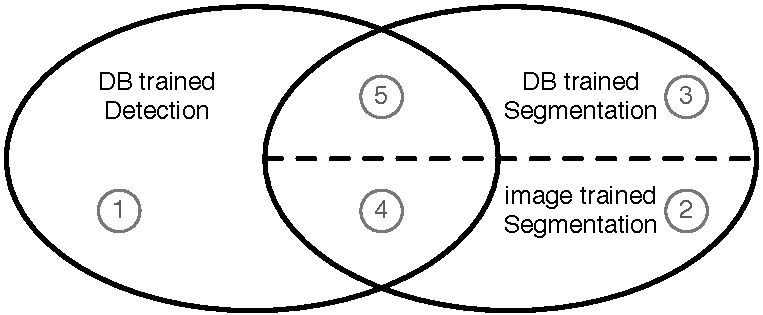
\includegraphics[width=.8\textwidth]{MLtypes}
\begin{tikzpicture}
	\def\scale{5.4}
    \draw (0,0) node [draw,ellipse,minimum height={\scale*1cm}, minimum width={\scale*1.618cm}] (a) {};
     \draw ({\scale*1.618*.5},0) node [draw,ellipse,minimum height={\scale*1cm}, minimum width={\scale*1.618cm}] (b) {};
     \draw [dashed] ($(b.east)$) -- ($(b.west)$)
    ($(a.north west)$) node [align=center,fill=white,inner sep=0pt,outer sep=0pt] {DB Trained\\ Detection}
    ($(b.north east)$) node [align=center,fill=white,inner sep=0pt,outer sep=0pt]{DB Trained\\ Segmentation}
    ($(b.south east)$) node [align=center,fill=white,inner sep=0pt,outer sep=0pt]{Image Trained\\ Segmentation};
	  
    \draw 	(-1.9,-1) node [] {\color{autoGuided}Madabhushi et al. [2003]}%\cite{Madabhushi:2003p6036}}
			 	(-1.8,.7) node []{\color{autoGuided}Massich et al.}
			 	(-1.8,.25) node []{\color{autoGuided}[2010, 2011, 2012]}%\cite{massich2010lesion,massich2011seed,massich2012seed}}
			 	(6.5,-.5) node []{\color{semiAuto}\cite{Xiao:2002p5639}}%,gerard2013}}
			 	(6.5,.5) node []{\color{autoGuided}\cite{Shan:2012p14347}}
			 	(5.8,1) node [] {\color{fullyAuto}\cite{Liu:2010p12036}}
			 	(2,.4)node []{\color{autoGuided}\cite{Zhang:2010p14317}}
			 	(2,-.7)node []{\color{fullyAuto}\cite{hao2012combining}}
			 	(6,-1)node[]{\color{semiAuto}\cite{chiang2010cell}}
			 	(2.1,.9)node []{\color{autoGuided}\cite{Jiang:2012p14354}};

\end{tikzpicture}

\caption[Conceptual map of supervised \ac{ml} training and goals.]{Supervised \acf{ml} training and goals, ending up with a combination of 5 different strategies. The references are colored indicating the user interaction: semi-automatic {\color{semiAuto}\semiAutoColor}, auto-guided{\color{autoGuided}\autoGuidedColor}, and fully automatic{\color{fullyAuto}\fullyAutoColor}.}
\label{fig:mltypes}
\end{figure}


\begin{description}
\item[Database Trained Detection:] generates statistic models from a training dataset to detect lesions in a target image using any sort of \ac{ml} and features~\cite{massich2010lesion,massich2011seed,massich2012seed,Madabhushi:2003p6036,Zhang:2010p14317,Jiang:2012p14354,hao2012combining}.
%In this case, usually low-level features such as intensity or texture descriptors~\cite{massich2010lesion,massich2011seed,massich2012seed,Madabhushi:2003p6036} are being used. 
%However more sophisticated detection methodologies like the ones proposed in Hao et al.~\cite{hao2012combining} could be used.
\item[Image Trained Segmentation:] from information supplied by the user, an \ac{ml} procedure is trained from the target image in order to produce a segmentation~\cite{Xiao:2002p5639,gerard2013}.
\item[Database Trained Segmentation:] the statistic models generated from the dataset are not used for localizing the lesion but rather to perform the segmentation itself. These methodologies produce image segmentation with no user interaction~\cite{Liu:2010p12036,Shan:2012p14347}. In such a scenario, the features for constructing the models need to be robust to significative differences between the images.
\item[Database Trained Detection and Image Trained Segmentation:]  
 \hfill \\
detection and segmentation are performed in a daisy chain manner like the models from a training dataset facilitate the detection of lesions within a target image. Once the suspicious areas are detected, they are used to train another \ac{ml} procedure within the target image to drive the final segmentation. Although the errors in the detection step are propagated,  this approach has the advantage that the statistical model driving the final segmentation has been specially built for every target image. The main drawback is that building this statistical model involves a training stage which is computationally very expensive~\cite{Zhang:2010p14317,Jiang:2012p14354}.
\item[Integrated Methodology:]  trying to take advantage of the detection without building a specific model for the target image. Since there is no need to make the final detection decision weather there is a lesion or not, the posterior probability of the decision process can be used as another feature like a filter response of the image and integrated with the \ac{ml} procedure~\cite{hao2012combining}.
\end{description}

%Here, the differences between the last three classes (automatic segmentation using \ac{ml}) are discussed in a generic manner. Although particularities of all different learning techniques implemented to achieve the goal might differ what is here said, the reflection here carried out only intents to transmit a global idea which aforesaid it might not be adequate for some particular implementations.
%Database learning seeks a more generic target meanwhile image training can better cope with inhomogeneities within the images (sonification problems) since the appearance of the lesion is inferred from the target image itself. 
%
%Database driven segmentation use generic stochastic models obtained from a training dataset forcing the features to be robust to inhomogeneities between the images.
%The advantage of using a database driven detection to initialize a image driven segmentation model is that a generic model based on a training dataset is used to detect the lesions and from this an stochastic lesion model for the specific target image is build in order to obtain more accurate results. The main drawback is that a training stage (which is the computationally expensive part of using \ac{ml}) needs to be carried out for every target image. 
%Integrated methodologies however try to take advantage of the detection without building an specific model for the target image. Since there is no need of taking the final detection decision whereas it is a lesion or not, the posterior of the decision process can be used as another feature like a filter response of the image and integrated with the \ac{ml} procedure.

%and adapted to address different parts of the problem. 
%In this field machine learning is widely used and intended to tackle different problems. It can be used to generate a segmentation by training within the same target image whether the training information is supplied by a user~\cite{Xiao:2002p5639} or automatically~\cite{Zhang:2010p14317,Jiang:2012p14354}.  
%
%  like lesion detection, segmentation, 
%Machine learning are widely used and the features are diverse, but here it is wanted to mention the difference between hao2012combining

\subsection{Others}

Here are listed other methods or parts of methods that are neither explicitly \ac{acm} nor \ac{ml} procedures, nor are they basic image processing or image analysis techniques such as thresholding or region growing. In this sense, three main groups can be identified:

\begin{itemize}
\item{\acf{gcs} based methods}
\item{unsupervised learning and over segmentation}
\item{disk expansion for image inpainting}
\end{itemize}

Methods using \ac{gcs} for segmenting breast lesions in \ac{us} data~\cite{Horsch:2001p6028,massich2010lesion,Drukker:2002p10442,Gomez:2010p14339}
 are inspired by the work of Kupinski et al.~\cite{Kupinski:1998p9024} which was initially adapted to \ac{us} data by Horsch et al.\cite{Horsch:2002p6049}. They are based on constraining a multivariate Gaussian function with an image dependent function so that, when the resulting function is thresholded, a possible delineation is generated. Although these methodologies are not posted in the \ac{acm} form, they are equivalent to a fast marching LevelSet procedure~\cite{sethian1996fast}. Thresholding can be seen as a contour propagation, while the Gaussian constraining forces the direction of the propagation to be constant. 

Some methods split the image or over-segment them for further operations like contour initialization~\cite{Huang:2005p11636,Huang:2012p14313} or higher level features extraction from a coherent area so that it can be used in \ac{ml} procedures~\cite{hao2012combining,chiang2010cell}. In order to carry out such an operation from a \ac{ml} point of view, several unsupervised learning techniques have to be used in order to group the pixels: fuzzy C-means, K-means~\cite{Cui:2009p14325}, and robust graph based clustering~\cite{Huang:2012p14313}. 
From an image analysis point of view, the grouping of similar contiguous pixels is equivalent to performing an over-segmentation of the image. Watershed transform~\cite{Huang:2005p11636,chiang2010cell,Huang:2004p2092} and \ac{nc}~\cite{shi2000normalized,hao2012combining,Liu:2005p14341} are popular techniques used to obtain an over-segmentation, also known as super pixels~\cite{achanta2012slic}. 

Finally, Yeh et al.~\cite{Yeh:2009p11985} proposed a totally different approach for breast lesion segmentation based on inpainting of degraded typology. The image is transformed into a binary image using local thresholding and then the largest object within the binary image is reconstructed as the final segmentation.

\subsection{Features}
Intensity remains the most used feature within the methods analyzed. A feasible explanation might be found in the difficulty of incorporating other features rather than intensity or its gradient in the \ac{acm} procedures. 
A way to incorporate features other than intensity, such as texture, within the process is proposed by Aleman-Flores et al.~\cite{AlemanFlores:2007p14310}.
The segmentation is carried out as two \acp{acm} connected in a daisy chain manner. The second \ac{acm} evolves through the target image, whereas the first \ac{acm} used to obtain a preliminary segmentation evolves using a generated image encoding the texture. This image is obtained by processing the target image using a modified anisotropic smoothing driven by texture features. The \ac{acm} evolves towards the gradient of this generated image already encoding texture information.

Texture descriptors have been more widely explored for methodologies incorporating \ac{ml} since these methodologies naturally deal with multiple features. However, texture description is highly dependent on the scale of the features and seeing speckle as image texture is arguable since speckle is an unwanted effect that depends on the characteristics of the screening tissue, the acquisition device and its configuration~\cite{Ensminger:2008p6920}. However, images does look like a combination of texture granularities depending on the tissue which has encouraged the exploration of texture descriptors~\cite{massich2010lesion,massich2011seed,massich2012seed,Madabhushi:2003p6036,Liu:2012p14316,hao2012combining,Huang:2005p11636}. However, the use of a naive descriptor, like the one used in \cite{massich2010lesion,massich2011seed,Madabhushi:2003p6036}, cannot represent the large variability in texture present throughout the images. This can be qualitatively observed by comparing the \ac{map} of the intensity and texture features, as shown in figure~\ref{fig:texture}, where the latent information contained in the texture (fig.~\ref{fig:texture}b) is less than that contained in the intensity feature (fig.~\ref{fig:texture}a).
A solution to cope with such texture variability consists of exploring multiple texture descriptors at multiple scales at the expense of handling larger feature sets resulting in a higher computation complexity and data sparsity that need to be handled. 

On the other hand, texture can be seen as a filter response, so it performs the posterior of a classification process. Therefore, more sophisticated textures can be seen as the outcome of an \ac{ml} process. Hao et al.~\cite{hao2012combining} propose to synthesize texture from a lesion detection process (\ac{dpm}) that takes advantage of \ac{hog} taken at different scales. Figure~\ref{fig:texture}c illustrates the feature plane inferred from the \ac{dpm} process.


\begin{figure}[Htbp]
\centering
\subfloat[]{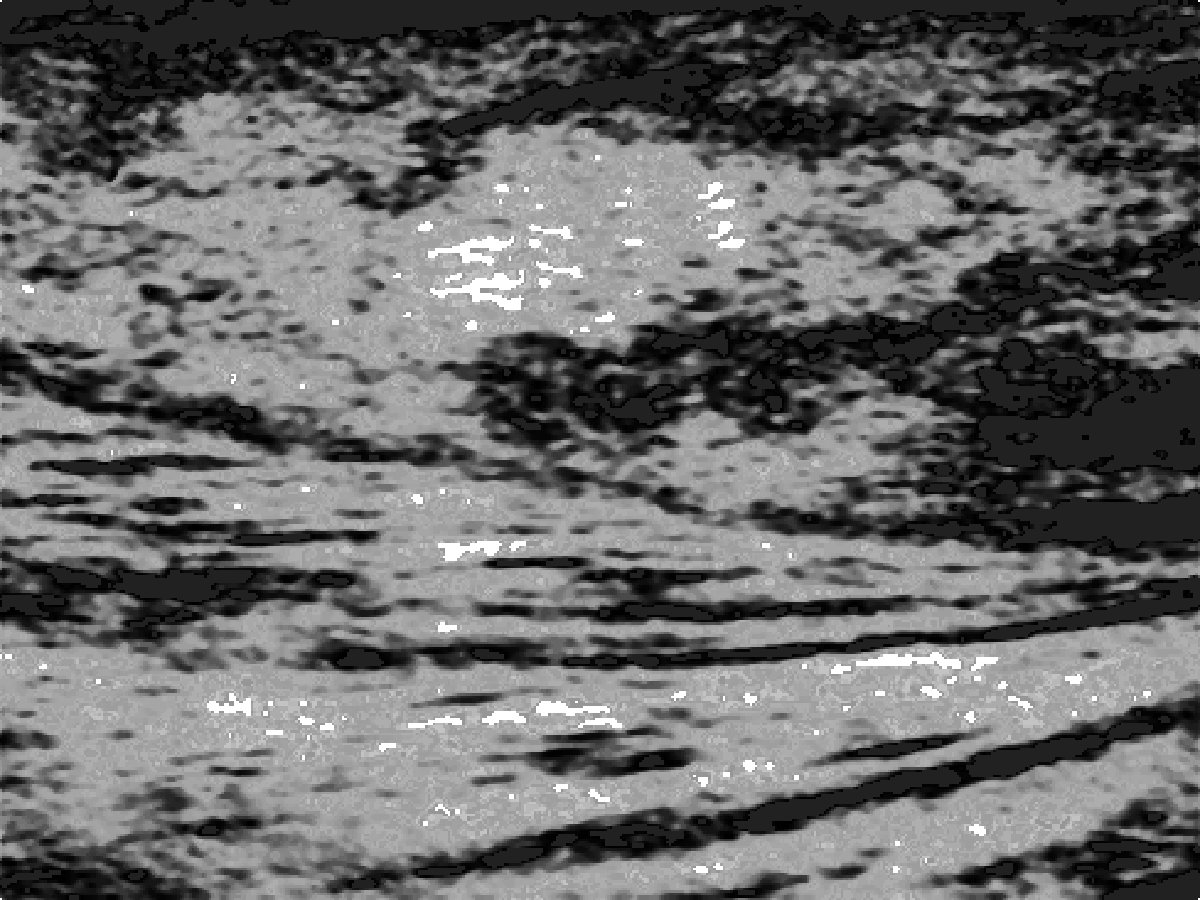
\includegraphics[width=.3\textwidth]{iIntensityP}}\,
\subfloat[]{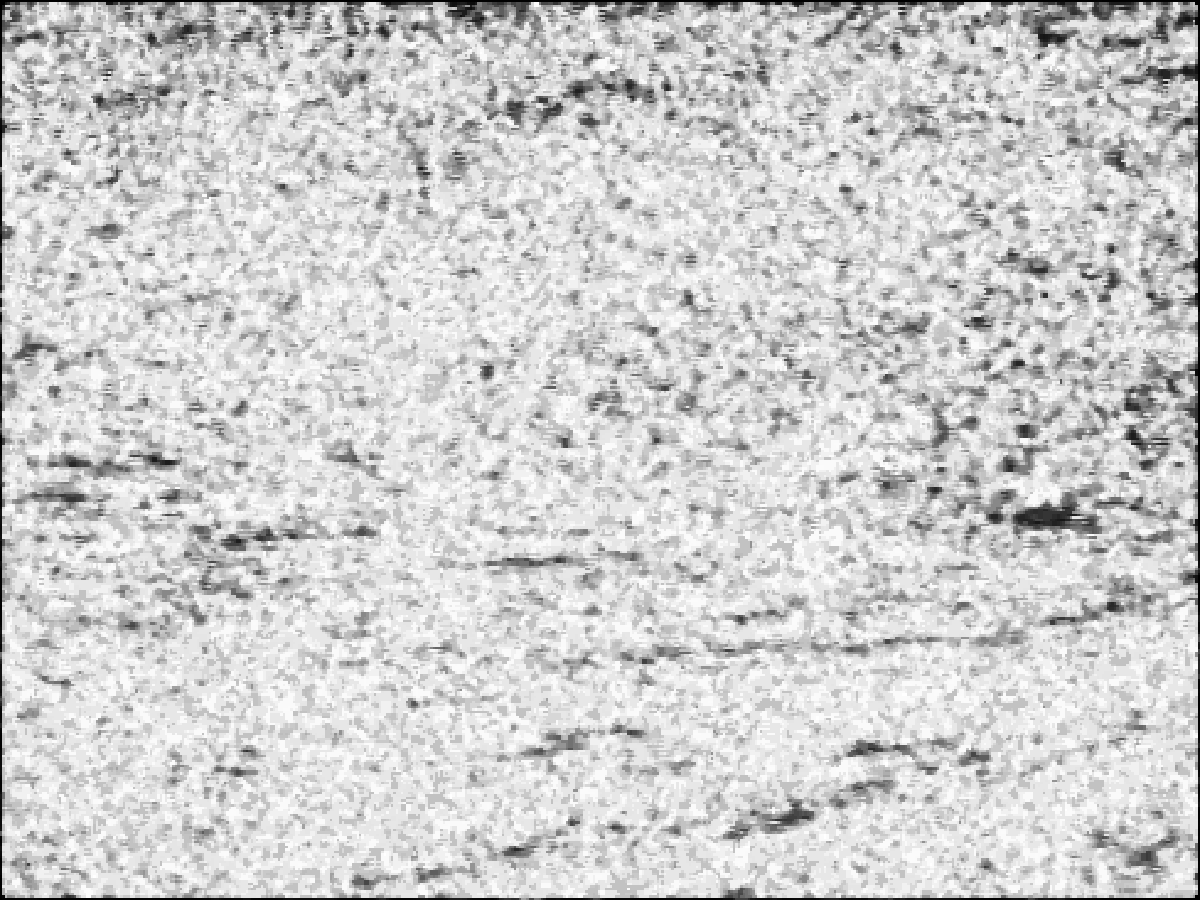
\includegraphics[width=.3\textwidth]{iTextureP.png}}\,
\subfloat[]{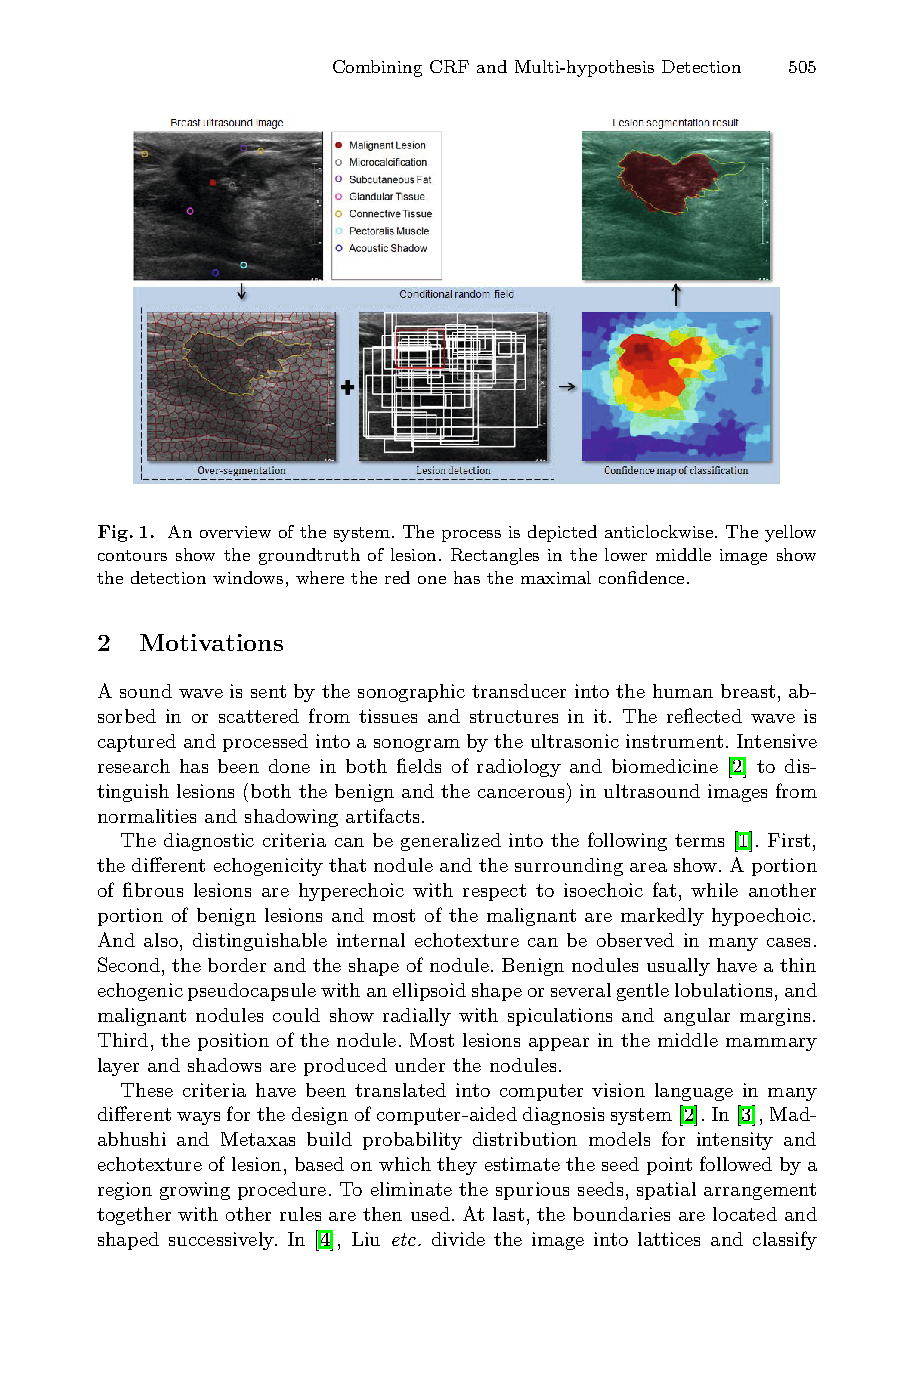
\includegraphics[trim = 99mm 157.8mm 25mm 54mm, clip,width=.3\textwidth]{TextureHao}}
\caption[Qualitative assessment of some feature examples]{Qualitative assessment of feature planes: (a) \acf{map} of intensity feature, (b) \ac{map} of texture feature used in~\cite{massich2010lesion,Madabhushi:2003p6036} and (c) quantified \ac{dpm} feature~\cite{hao2012combining}(image taken from the original work in~\cite{hao2012combining}).}
\label{fig:texture}
\end{figure}


 
\section{Segmentation assessment}\label{section:assessment}
Comparing all the methodologies reviewed in section~\ref{section:userInteraction} is rather cumbersome. The lack of a common framework for assessing the methodologies remains unaddressed, especially due to the absence of a public image dataset despite its being highly demanded by the scientific community~\cite{Noble:2006p1734,Noble:2009p14330,Cheng:2009p10580}. However, the lack of a common dataset is not the only aspect complicating the comparisons. Here is a list of some of the feasible aspects complicating direct comparison of the works reviewed.

\begin{itemize}
\item Uncommon database
\item Uncommon assessing of criteria and metrics
\item Different degrees of user interaction
\item Inability to quantify the user effort when interacting with a method
\item Correctness of the \ac{gt} used when assessing
\item Uncommon treatment of missegmentation due to unpropper detection
\end{itemize}

%The comparison of the segmentation performance of all the methods previously described, is rather cumbersome. Not only because they have been assessed using different sets of images, but also because the metrics being used for reporting the results also vary. Despite the need of a common framework for comparing methodologies for segmenting breast lesions in \ac{us} images is highly demanded by the scientific community~\cite{Noble:2006p1734,Noble:2009p14330,Cheng:2009p10580}, it still remains unaddressed. 
%
%Apart from images sets and metrics, the user interaction effort for interactive segmentations, the correctness of the \ac{gt} due to intra expert and inter expert variability on the segmentations~\cite{gerard2013} and the amount of missegmentation due to an unpropper detection are also difficult to assess and compare.


The dificulty of comparing the methodologies using distinct datasets, distinct assessing criteria and distinct metrics is clear. 
Section~\ref{section:evalCriteria} analyzes the criteria and metrics used to analyze the different methodology proposals. In order to conduct a discussion comparing the methodologies in section~\ref{discussion}, when enough information is available, the reported results are set to a common framework for comparison purposes despite being assessed with different datasets.
The assessment regarding user interaction is not further analyzed other than the already described interactive and automatic classification along with their respective subcategories (see section~\ref{section:userInteraction} and fig.~\ref{fig:segmentationInteractivityTable}). 
The correctness of the \ac{gt} for assessing the segmentations refers to the huge variability of the delineations found when analyzing intra expert and inter expert variability on the segmentations~\cite{gerard2013}. In this regard, later in this article (see section:~\ref{sec:multipleGT}), a short discussion about the work that took intra and inter-observer delineation variability into account for assessing segmentation proposals can be found. 
Finally, the frontier between segmentation errors and errors due to the detection process is unclear and a proper criterion is not set. Massich et al.~\cite{massich2010lesion} take all the segmentations into account even if the segmentation has been wrongly initialized by the automatic detection procedure. Meanwhile, Zhang et al.~\cite{Zhang:2010p14317} only use 90\% of the best segmentations to perform the segmentation assessment, arguing that the remaining segmentations suffered poor detection and that segmentation result assessment should not be subject to wrong initializations.

%Regarding interaction effort, for the work presented  here, user interactivity assessing is only based whether the methodologies are interactive or automatic (see fig.~\ref{fig:segmentationInteractivityTable}). 
%Regarding the correctness of the \ac{gt} further in this chapter (see section:~\ref{sec:multipleGT}) can be found a little discussion about the works that took intra and inter-observer delineations variability into account for assessing segmentation proposals. 
%Finally the frontier between segmentation errors and errors due to the detection process is unclear and a proper criteria is not set. Massich et al.~\cite{massich2010lesion} take all the segmentations into account even if the segmentation has been wrongly initialized by the automatic detection procedure. Meanwhile, Zhang et al.~\cite{Zhang:2010p14317} only uses the best 90\% of the segmentations to perform the segmentation assessment arguing that the remaining segmentations suffered a poor detection and that segmentation results assessment should not be subject to wrong initializations.

The rest of this section describes different area and boundary metrics collected from the works cited above,  comments on the correctness of the assessing \ac{gt}, based on intra- and inter-observer \ac{gt}, variability and discusses the results reported.

\subsection{Evaluation criteria}\label{section:evalCriteria}
Although multiple criteria arise when assessing segmentations, these criteria can be grouped into two families depending on whether they are area or distance based metrics as illustrated in figure~\ref{fig:gtEval}. Area based metrics assess the amount of area shared (\acf{aov}) between the obtained segmentation and the reference. On the other hand, distance based metrics quantify the displacement or deformation between the obtained and the desired delineations. 

For the sake of simplicity, the name of the reported similarity indexes has been unified.

\begin{figure}[Htbp]
\centering

\subfloat[]{
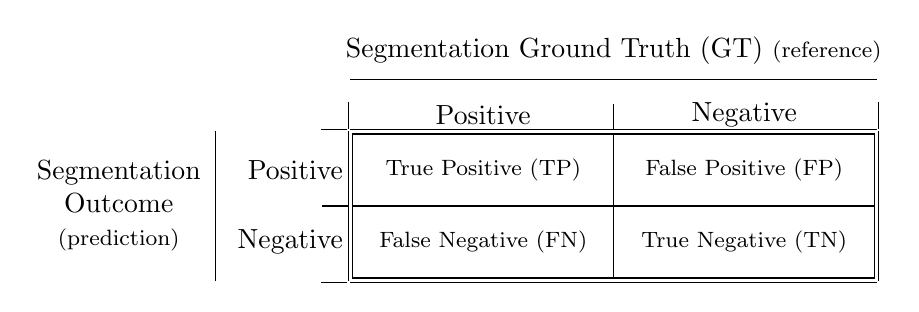
\begin{tikzpicture}[node distance= 0 and 0]
\def\scale{1.5}
\tikzstyle{bk}=[font=\footnotesize,minimum height={\scale*.6cm}, minimum width={\scale*2.2cm}]
\tikzstyle{bklabel}=[]
\tikzstyle{bkaux}=[font=\footnotesize,inner sep=0pt,outer sep=0pt]

\draw node[bk](tp){True Positive (TP)}
		   node[ bk, right =of tp] (fp) {False Positive (FP)}
		   node[ bk, below =of fp] (tn) {True Negative (TN)}
		   node[ bk, left =of tn] (fn) {False Negative (FN)}
		   
		   node[bklabel,above =of tp] (p)  {Positive}
  		   node[bklabel] at ( p -| fp) {Negative}
		   (tp.west) node[bklabel,left] (xx) {Positive}
  		   (fn.west) node[bklabel,left] {Negative}
;
\draw 	(tp.north west) -- (fp.north east) -- (tn.south east) -- (fn.south west) -- cycle
			(tp.south west) -- (fp.south east)     (tp.north east) -- (fn.south east);
			
% get auxiliar positions and drawing the lines
\def\separation{1pt}
\def\segmentlength{10pt}
\draw	node [bkaux,above left	= \separation and \separation of tp](a){}
			node [bkaux,above right	= \separation and \separation of fp](b){}
			node [bkaux,below right	= \separation and \separation of tn](c){}
			node [bkaux,below left	= \separation and \separation of fn](d){}
			(tp.north east)	++(0,\separation) node [bkaux](e){}
			(tp.south west)	++(-\separation,0) node [bkaux](f){};

\draw (a) -- (b) -- (c) -- (d) -- (a);
\draw (a) -- ++(0,\segmentlength) 	(e) --	++(0,\segmentlength)	(b) -- ++(0,\segmentlength);
\draw (a) -- ++(-\segmentlength,0)	(f) --		++(-\segmentlength,0)	(d) -- ++(-\segmentlength,0);

% draw the GT / segmentation labels
\draw node [bkaux,left = {\scale*1.1cm} of a] (g) {} 
		   node [bkaux,left = {\scale*1.1cm} of d] (h) {}
		   node [bkaux,left = \separation of g] (i) {} 
		   node [bkaux,left = \separation of h] (j) {}		   
		   (g) -- (h)  %(i) -- (j)
		   
		   node [bkaux,above = {\scale*.4cm} of a] (k) {} 
		   node [bkaux,above = {\scale*.4cm} of b] (l) {}
		   node [bkaux,above = \separation of k] (m) {} 
		   node [bkaux,above = \separation of l] (n) {}		   
		   (k) -- (l)  %(m) -- (n) 
		   
		   ($ (i) !.5! (j) $) node[bklabel,align=center,left] {Segmentation \\ Outcome \\{\footnotesize(prediction)}}
		   ($ (m) !.5! (n) $) node[bklabel,align=center,above] {Segmentation Ground Truth (GT) {\footnotesize(reference)}}
;
\end{tikzpicture}
}%end sufloat
\\
\subfloat[]{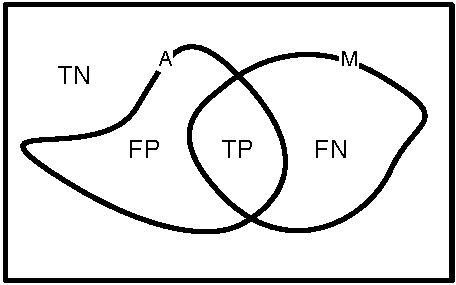
\includegraphics[height=.3\textwidth]{aor}}~
\subfloat[]{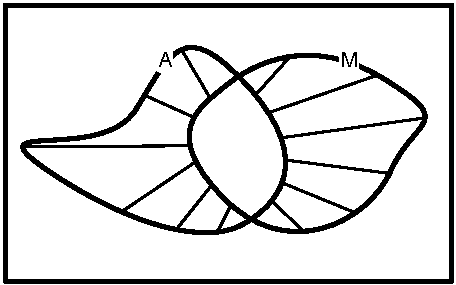
\includegraphics[height=.3\textwidth]{disterror}}
\caption[Methodology evaluation.]{ Methodology evaluation. (a) Statistical hypothesis test errors confusion matrix. (b) 
Graphic representation of the statistical hypothesis test errors for assessing the performance in terms of area. (c) Graphical representation of the boundary distance performance measures.}
\label{fig:gtEval}
\end{figure}

\subsubsection{Area based segmentation assessment metrics}
%When analyzing the areas described by the assessing segmentation $A$ and the reference segmentation $M$ (see fig.~\ref{fig:gtEval}b), 4 regions become apparent: \acf{tp},  \acf{tn},  \acf{fp},  and \acf{fn}; corresponding to the regions of the confusion matrix in figure~\ref{fig:gtEval}a.

When analyzing the areas described by the segmented region  to be assessed, $A$ and the manually delineated reference region $M$ (see fig.~\ref{fig:gtEval}b), 4 areas become evident: \acf{tp},  \acf{tn},  \acf{fp},  and \acf{fn}; corresponding to the regions of the confusion matrix in figure~\ref{fig:gtEval}a.


%\begin{table}[htdp]
%\caption{Statistical hypothesis test errors confusion matrix}
%\begin{center}
%\begin{tabular}{r||c|c|}
%&Positivie & Negative \\ \hline \hline
%Poisitve & \acf{tp} & \acf{fp}\\ \hline
%Negative & \acf{fn} & \acf{tn}\\
%\hline \hline
%\end{tabular}
%\end{center}
%\label{fig:TPTNconfusionMatrix}
%\end{table}%



%%
%%\begin{description}
%%\item[\acf{tp}]
%\paragraph{\acf{tp}}
%is found as the area in common ($A \wedge M$) between the two delineations $A$, $M$. 
%The \ac{tp} area corresponds to the correctly segmented areas belonging to the lesion.
%
%%\item[\acf{tn}] 
%\paragraph{\acf{tn}}
%is found as the area ($\overline{A} \wedge \overline{M}$) not belonging to either of the delineations $A$ nor $M$ . The \ac{tn} area corresponds to the correctly segmented areas belonging to the background of the image. 
%
%%\item[\acf{fp}] 
%\paragraph{\acf{fp}}
%is found as the area ($A \wedge \overline{M}$) belonging to the assessing segmentation $A$ and not as a part of the reference delineation $M$. \ac{fp} corresponds to the area wrongly labeled as a lesion since this area does not belong to the reference delineation.
%
%%\item[\acf{fn}] 
%\paragraph{\acf{fn}}
%is found as the area ($\overline{A} \wedge M$) corresponding to the reference delineation $M$ but not as a part of the assessing segmentation $A$. \ac{fn}
%corresponds to the areas of the true segmentation that have been missed by the segmentation under assessment.

%\end{description}
\vspace{15pt}
Area metrics (or indexes) for assessing the segmentation are defined as a dimensionless quotient relating the 4 regions (\ac{tp}, \ac{fp}, \ac{fn} and \ac{tn}) described by the segmentation outcome being assessed (denoted $A$ in fig:\ref{fig:gtEval}a) and the reference \ac{gt} segmentation (denoted $M$). Most of the indexes are defined within the interval $[0,1]$ and some works report their results as a percentage.

\begin{description}

\item[\acf{aov},] also known as overlap ratio, the \ac{jsc}~\cite{Gao:2012p14336} or \ac{si}~\cite{Shan:2012p14347}\footnote{Notice that \acf{si} is also used formulated as the \acf{dsc} in~\cite{Huang:2007p6100,Huang:2005p11636} which differs from the \ac{si} definition in~\cite{Shan:2012p14347}.}, is a common similarity index representing the percentage or amount of area common to the assessed delineation $A$ and the reference delineation $M$ according to equation~\ref{eq:aov}. 
The \ac{aov} metric has been used to assess the following works: \cite{Horsch:2001p6028,Gomez:2010p14339,AlemanFlores:2007p14310,Cui:2009p14325,massich2010lesion,Shan:2012p14347,hao2012combining,Liu:2010p14328}

\begin{equation}\label{eq:aov}
AOV = \frac{TP}{TP+FP+FN}=\frac{|A| \wedge |M|}{|A| \vee |M|} \qquad \in [0,1]
\end{equation}

\item[\acf{dsc},]
also found under the name of \ac{si}~\cite{Huang:2007p6100,Huang:2005p11636}\footnote{Notice that \acf{si} is also used formulated as the \acf{aov} in~\cite{Shan:2012p14347} which differs from the \ac{si} definition in~\cite{Huang:2007p6100,Huang:2005p11636}.},
is another widely used overlap metric similar to \ac{aov}. The difference between \ac{dsc} and \ac{aov} is that \ac{dsc} takes into account the \ac{tp} area twice, one for each delineation. 
The \ac{dsc} index is given by equation~\ref{eq:dsc} and the relation between \ac{aov} or \ac{jsc} and the \ac{dsc} similarity indexes is expressed by equation~\ref{eq:dsc2jsc}. Notice that the \ac{dsc} similiarity index is expected to be greater than the \ac{aov} index~\cite{gerard2013}. The \ac{dsc} metric has been used to assess the following works:\cite{gerard2013,Huang:2007p6100,Zhang:2010p14317,Huang:2005p11636}

\begin{equation}\label{eq:dsc}
DSC=\frac{2 \cdot TP}{2 \cdot TP + FP + FN}=\frac{2 | A \wedge M |}{|A| + |M|} \qquad \in [0,1]
\end{equation}

\begin{equation}\label{eq:dsc2jsc}
DSC=\frac{2 \cdot AOV}{1+AOV}
\end{equation}

\item[\acf{tpr},]
also known as the recall rate, sensitivity (at pixel level)~\cite{gerard2013,Jiang:2012p14354} or \ac{of}~\cite{Huang:2007p6100}, quantifies the amount of properly labeled pixels as lesion with respect to the amount of lesion pixels from the reference delineation (eq:~\ref{eq:tpr}). Notice that like the \ac{dsc}, this value always remains greater than \ac{aov} (or equal when the delineations are identical). The \ac{tpr} metric has been used to assess the following works:~\cite{Madabhushi:2003p6036,Huang:2007p6100,Shan:2012p14347,Jiang:2012p14354,Huang:2005p11636,Huang:2012p14313,Liu:2010p14328,Yeh:2009p11985}


\begin{equation}\label{eq:tpr}
TPR = \frac{TP}{TP+FN}= \frac{TP}{|M|} = \frac{|A| \wedge |M|}{|M|} \qquad \in [0,1]
\end{equation}

\item[\acf{ppv}]
corresponds to the probability that the pixel is properly labeled when restricted to those with positive test. It differentiates from \ac{tpr} since here the \ac{tp} area is regularized by the assessing delineation and not the reference, as can be seen in equation~\ref{eq:ppv}. \ac{ppv} is also greater than \ac{aov}. The \ac{ppv} metric is also used to assess the work in~\cite{gerard2013}.

\begin{equation}\label{eq:ppv}
PPV= \frac{TP}{FP+TP} = \frac{TP}{|A|}=\frac{|A| \wedge |M|}{|A|} \qquad \in [0,1]
\end{equation}


\item[\acf{nrv},]
also found as the Precission Ratio(PR)~\cite{Huang:2004p2092}, corresponds to the area of disagreement between the two delineations regularized by the size of the reference delineation, as described in equation:~\ref{eq:nrv}. Notice that the \ac{nrv} coefficient differs from $1-\ac{aov}$ since it is regularized by the reference delineation and not the size of the union of both delineations.
The \ac{nrv} metric has been used to assess the following works:~\cite{Gomez:2010p14339,Liu:2005p14341,Huang:2004p2092}.


\begin{equation}\label{eq:nrv}
NRV = \frac{|A \oplus M|}{|M|} \qquad \in \left[0, 1+\frac{A}{|M|}\right]
\end{equation}


\item[\acf{fpr},]
as reported in the presented work, is the amount of pixels wrongly labeled as lesion with respect to the area of the lesion reference, as expressed in equation~\ref{eq:fpr}. The \ac{fpr} metric has been used to assess the following works:\cite{Madabhushi:2003p6036,Shan:2012p14347,Huang:2012p14313,Liu:2010p14328,Yeh:2009p11985} The \ac{fpr} has also been found in its complementary form $1-TPR$ under the name of Match Rate (MR)~\cite{Huang:2004p2092}.

\begin{equation}\label{eq:fpr}
FPR'= \frac{FP}{TP + FN} = \frac{FP}{|M|}=\frac{|A \vee M - M|}{|M|} \qquad \in \left[0,\frac{A}{|M|}\right]
\end{equation}

Notice that the \ac{fpr} calculated in equation~\ref{eq:fpr} differs from the classic \ac{fpr2} obtained from the table in figure~\ref{fig:gtEval}a, which corresponds to the ratio between \ac{fp} and its column marginal ($FP+TN$), as indicated in equation~\ref{eq:fpr2}. The \ac{fpr2}, when calculated according to equation~\ref{eq:fpr2}, corresponds to the complement of specificity (described below).

\begin{equation}\label{eq:fpr2}
FPR= \frac{FP}{FP + TN} = 1-SPC \qquad \in [0,1]
\end{equation}

\item[\acf{fnr}]
corresponds to the amount of pixels belonging to the reference delineation that are wrongly labeled as background, as expressed in equation~\ref{eq:fnr}. Notice that it also corresponds to the inverse of the \ac{tpr} since $TP \cup FN = M$.
The \ac{fnr} metric has been used to assess the following works:
\cite{Madabhushi:2003p6036,Huang:2012p14313,Yeh:2009p11985}

\begin{equation}\label{eq:fnr}
FNR = \frac{FN}{|M|}=\frac{|A \vee M - A|}{|M|}=1-TPR \qquad \in [0,1]
\end{equation}

\item[Specificity] corresponds to the amount of background correctly labeled. Specificity is described in equation~\ref{eq:specificity} and is usually given as complementary information on the sensitivity (\ac{tpr}). Specificity corresponds to the complementary of the \ac{fpr2} when calculated according to equation~\ref{eq:fpr2}. The specificity index is also used to assess the work in~\cite{gerard2013,Jiang:2012p14354}.

\begin{equation}\label{eq:specificity}
SPC = \frac{TN}{TN+FP} = \frac{|\overline A \wedge \overline M|}{|\overline M|}=1-FPR \qquad \in [0,1]
\end{equation}
\end{description}

\subsubsection{Boundary based segmentation assessment metrics}

Although the boundary assessment of the segmentations is less common than area assessment, it is present in the following works: \cite{AlemanFlores:2007p14310,Gomez:2010p14339,Gao:2012p14336,Madabhushi:2003p6036,
Shan:2012p14347,Zhang:2010p14317,Huang:2012p14313}. Like when assessing the segmentations in terms of area, the criteria for assessing disagreement between outlines are also heterogeneous which makes the comparison between works difficult. 
Unlike the area indexes, with the exception of the further introduced \ac{are} coefficient, which is also a dimensionless quotient, the rest of the boundary indexes or metrics are physical quantitative error measures and are assumed to be reported in pixels. Although some of the reported measures are normalized, they are not bounded by any means.

Zhang et al.~\cite{Zhang:2010p14317} propose using average contour-to-contour distance ($E_{cc}$) for assessing their work. However, no definition or reference is found on it. Huang et al.~\cite{Huang:2012p14313} propose using \ac{are}, defined in equation~\ref{eq:are}, where a set of $n$ radial rays are generated from the center of the reference delineation $C_0$ intersecting both delineations. The \ac{are} index consists of averaging the ratio between the distance of the two outlines $|C_s(i)-C_r(i)|$ and the distance between the reference outline and its center $|C_r(i)-C_0|$.

\begin{equation}\label{eq:are}
ARE = \frac{1}{n}\sum_{i=1}^{n} \frac{|C_s(i)-C_r(i)|}{|C_r(i)-C_0|}
\end{equation}

The rest of the works base their similitude indexes on the analysis of the \ac{md} coefficients. The \ac{md} is defined in equation~\ref{eq:md} and corresponds to the minimum distance between a particular point $a_i$ within the contour $A$ (so that $a_i \in A$) and any other point within the delineation $M$. 

\begin{equation}
\text{MD}(a_i,M) =\min_{m_j \in M}\Arrowvert a_i - m_j \Arrowvert 
\label{eq:md}
\end{equation}

\paragraph{\acf{hd},} or Hausdorff error, measures the worst possible discrepancy between the two delineations $A$ and $M$ as defined in \ref{eq:Hd}. Notice that it is calculated as the maximum of the worst discrepancy between $(A,M)$ and  $(M,A)$ since \ac{md} is not a symmetric measure, as can be observed in figure~\ref{fig:md}. The \ac{hd} as defined in equation~\ref{eq:Hd} has been used for assessing the segmentation results in Gao et al.~\cite{Gao:2012p14336}. Meanwhile, Madabhushi and Metaxas~\cite{Madabhushi:2003p6036} and Shan et al.~\cite{Shan:2012p14347} only take into account the discrepancy between the assessed delineation $A$ with reference delineation $M$, here denoted as \ac{hd}' (see eq.\,\ref{eq:Hd2}). In \cite{Madabhushi:2003p6036,Shan:2012p14347}, the \ac{hd}' is also reported in a normalized form $\frac{\text{HD}'}{\eta}$, where $\eta$ is the length of the contour of reference $M$.

\begin{equation}
\text{HD} (A,M) = \max \bigg \{ \max_{a_i \in A} \text{MD}(a_i,M), \max_{m_i \in M} \text{MD}(m_i,A)  \bigg \}
\label{eq:Hd}
\end{equation}
\begin{equation}
\label{eq:Hd2}
\text{HD'} (A,M) = \max_{a_i \in A} \text{MD}(a_i,M)
\end{equation}

\begin{figure}[Htbp]
\centering
\subfloat[]{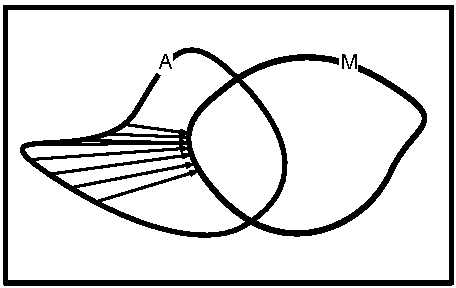
\includegraphics[height=.3\textwidth]{mdA-M}}~
\subfloat[]{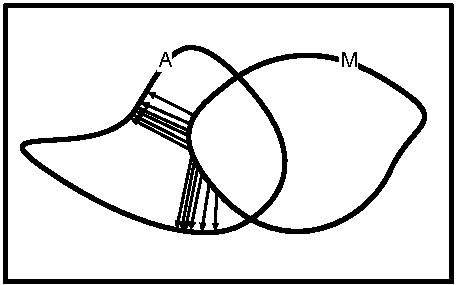
\includegraphics[height=.3\textwidth]{mdM-A}}

\caption[Non-symmetry propoerty of the \ac{md} metric.]{Illustration of the non-symmetry property of the \acf{md} metric. (a) $\text{MD}(a_i,M)$, (b) $\text{MD}(m_i,A)$}
\label{fig:md}
\end{figure}

\paragraph{\acf{amed},} defined in equation~\ref{eq:amed}, is the average \ac{md} between the two outlines.~\cite{Gao:2012p14336}. Similar to the case of the \ac{hd}' distance, Madabhushi and Metaxas~\cite{Madabhushi:2003p6036} and Shan et al.~\cite{Shan:2012p14347} only take into account the discrepancy between the assessed delineation $A$ with reference to the delineation $M$ to calculate the \ac{amed}' index (see eq.\,\ref{eq:amed2}). The \ac{amed} index can be found under the name of Mean Error (ME) in~\cite{Madabhushi:2003p6036} and Mean absolute Distance (MD) in.~\cite{Shan:2012p14347}.

\begin{equation}
\text{AMED} (A,M) = \frac{1}{2}  \cdot  \Bigg [ 
 \frac{ \sum_{a_i \in A} \text{MD}(a_i,M)}{|A|} + \frac{ \sum_{m_i \in M} \text{MD}(m_i,A) }{|M|} \Bigg ]
\label{eq:amed}
\end{equation}
\begin{equation}
\label{eq:amed2}
\text{AMED'} (A,M)= \frac{ \sum_{a_i \in A} \text{MD}(a_i,M)}{|A|}
\end{equation}

\paragraph{\ac{pd},} used in~\cite{AlemanFlores:2007p14310,Gomez:2010p14339}, takes into account the \ac{amed} regularized with the area of the reference delineation according to equation~\ref{eq:pd}

\begin{equation}
\text{PD} (A,M) = \frac{1}{2 \sqrt{\frac{Area(M)}{\pi}}} \cdot  \Bigg [ 
 \frac{ \sum_{a_i \in A} \text{MD}(a_i,M)}{|A|} + \frac{ \sum_{m_i \in M} \text{MD}(m_i,A) }{|M|} \Bigg ] * 100
\label{eq:pd}
\end{equation}

\subsection[Multiple grader delineations ]{Multiple grader delineations ( Study of inter- and intra-observer segmentation variability)}\label{sec:multipleGT}
%\footnote{\color{red} I swear God that i had a paper using a metric that takes into account two (and only two) graders GT. But i don't find it !!!}

Assessing the true performance of a medical imaging segmentation procedure is, at least, difficult. Although method comparison can be achieved by assessing the methodologies with a common dataset and metric, true conclusions about the performance of the segmentation are questionable. Assessing segmentations of medical images is challenging because of the difficulty of obtaining or estimating a known true segmentation for clinical data. Although physical and digital phantoms can be constructed so that reliable \ac{gt} are known, such phantoms do not fully reflect clinical imaging data. An attractive alternative is to compare the segmentations to a collection of segmentations generated by expert raters. 

Pons et al.~\cite{gerard2013} analyzed the inter- and intra-observer variability of manual segmentations of breast lesions in \ac{us} images. In the experiment, a subset of 50 images is segmented by an expert radiologist and 5 expert biomedical engineers with deep knowledge of a breast lesion appearance in \ac{us} data. The experiment reported an \ac{aov} rate between $0.8$ and $0.852$ for the 6 actors. This demonstrates the large variability between \ac{gt} delineations; a fact that needs to be taken into account in order to draw proper conclusions about the performance of a segmentation methodology. However, having multiple \ac{gt} delineations to better assess the segmentations performance is not always possible. When possible, several strategies have been used to incorporate such information.

Cui et al.~\cite{Cui:2009p14325} tested the segmentation outcome against 488 images with two delineations provided by two different radiologists. The dataset is treated as two different datasets and the performance on both is reported.
Yeh et al.~\cite{Yeh:2009p11985} used a reduced dataset of 6 images with 10 different delineations accompanying each image. The performance for each image was studied in terms of reward average and variation of the 10 reference delineations.
Aleman-Flores et al.~\cite{AlemanFlores:2007p14310}, where a dataset of 32 image dataset with 4 \ac{gt} delineations provided by 2 radiologists (2 each) was available, assessed the segmentation method as if there were 128 ($32 \times 4$) images.

A more elaborate idea to estimate the underlying true \ac{gt} is proposed by Massich et al.~\cite{massich2010lesion} and Pons et al.~\cite{gerard2013}. Both works propose the use of \ac{staple} in order to determine the underlying \ac{gt} from the multiple expert delineations. \ac{staple} states that the ground truth and performance levels of the experts can be estimated by formulating the scenario as a missing-data problem, which can be subsequently solved using an \ac{em} algorithm. The \ac{em} algorithm, after convergence, provides the \acf{hgt} estimation that has been inferred from the segmentations provided by the experts as a probability map. Massich et al.~\cite{massich2010lesion} propose to assess the segmentation against a thresholded \ac{hgt} and weight the \ac{aov} index with the \ac{hgt}. The authors in~\cite{massich2010lesion} argued that apart from comparing the segmentation resulting from binarizing the greaders segmentation agreement, the amount of agreement the needs to be taken into account. This way, properly classifying a pixel with large variability within the graders produces less reward and miss classifying a pixel with great consensus penalizes.

\section{Discussion}\label{discussion}

As has been said all along in section~\ref{section:assessment}, accurate comparison of the segmentation methodologies from their proposal works is not feasible. The major inconveniencies are uncommon assessing datasets and inhomogeneous assessing criteria, but the fact that all the indexes for assessing segmentations seen in section~\ref{section:assessment} are made at the image level can also be added. Therefore, the statistics used for reporting the performance of segmentation methodologies at the dataset level might vary as well. Most of the works report their dataset performance as an average of the image assessment reward. Some works complement such information with minimal and maximal value~\cite{Gomez:2010p14339}, the standard deviation~\cite{AlemanFlores:2007p14310,Cui:2009p14325,Zhang:2010p14317,hao2012combining,Huang:2012p14313,Liu:2010p14328}, or median~\cite{AlemanFlores:2007p14310,hao2012combining}. Some other works prefer to report the distribution of their results graphically~\cite{massich2010lesion,Gao:2012p14336,Yeh:2009p11985}. Finally, in~\cite{Huang:2007p6100,Shan:2012p14347}, it is not specified which statistic has been used, although mean is assumed.

Despite all the mentioned inconveniences, information regarding performance of all the works presented here is gathered in table~\ref{table:segmentationperformance} and graphically displayed in figure~\ref{fig:performanceComparison} in order to analyze some trends. In table~\ref{table:segmentationperformance}, the works presented are grouped depending on the user interaction according to the four categories described in section~\ref{section:userInteraction} corresponding to: interactive segmentation (fully-guided and semi-automatic) and automatic segmentation (auto-guided and fully-automatic). For each method the size of the dataset, the number of different \ac{gt} delineations per image used to assess the methodology and the results in the original work are reported. If the assessment index is found under another name rather than the name used in section~\ref{section:assessment}, the name used here as a reference appears in brackets to homogenize the nomenclature in order to facilitate comparison.
Finally, when enough information is available,  an inferred \ac{aov} value, also to facilitate comparing the works is shown in the last column of the table.

%Only methods such that \ac{aov} is available or it can be inferred from the data available are reported in figure~\ref{fig:performanceComparison} since the data is only reported in terms of \ac{aov}.

Figure~\ref{fig:performanceComparison} displays only those methods where \ac{aov} was available or could be inferred from the reported data. These representations synthesize the methods' performance and the datasets used for the assessment in a single view. The different works are radially placed according to different criteria and the references are colored in terms of the user interaction categories defined in section~\ref{section:userInteraction}.The \ac{aov} appears in blue in percentage as well as graphically within a score circle. In this score circle, there is also presented the intra- and inter-observer variability segmentation results reported in~\cite{gerard2013} as a blue colored swatch within two dashed circles that represent the minimum and the maximum disagreement reported in the experiment.
The size of the dataset used for assessing the segmentation performance appears in red. In the center of the radial illustration, a 3 class categorization of the size of the dataset has been carried out. The 3 classes correspond to small (less than 50 images), medium (between 50 and 250 images) and large (more than 250 images).

Figure~\ref{fig:performanceComparison}a rearranges the works presented according to the categories shown in figure~\ref{fig:segTypeMap}; \ac{acm}, \ac{ml}, others, and their combination. 
This representation in sectors facilitates ascribing the importance of a particular segmentation type at a glance, since combinations of these are placed contiguous to the unaccompanied type. For readability purposes, methodologies combining aspects of these three categories (\cite{Madabhushi:2003p6036,Cui:2009p14325}) have been chosen to belong to the combination of the two categories best describing the method. 
So, Madabhushi and Metaxas~\cite{Madabhushi:2003p6036} is treated as a combination of \ac{ml} and \ac{acm}, and Cui et al.~\cite{Cui:2009p14325} as an \ac{acm} and other methodology combinations.
%Although Madabhushi and Metaxas~\cite{Madabhushi:2003p6036} uses the Stavros rule and region growing which both belong to the class labeled as other, the \ac{map} from a training step driving the Stavros rule qualifies the method to be considered as a combination of \ac{ml} and \ac{acm}. On the other end, Cui et al.~\cite{Cui:2009p14325} only uses the unsupervised \ac{ml} technique of k-means on the intensity plane which is easily exchangeable with a threshold procedure, qualifying for being classified as a combination of \ac{acm} and other methodologies.
Figure~\ref{fig:performanceComparison}b arranges the presented works according to the user interaction. 
Figure~\ref{fig:performanceComparison}c only takes into account the presented works that make use of \ac{ml} and are arranged according to the criteria exposed in section~\ref{sec:ml} (see fig:\ref{fig:mltypes}) plus the unsupervised methods. Finally, Figure~\ref{fig:performanceComparison}d represents the methodologies belonging to the \ac{acm} class, arranged by type (see fig:\ref{fig:segTypeMap} and section~\ref{sec:acms}). 

When analyzing the figures, an already stated observation arises while comparing the methodologies against the swatch representing the inter- and intra-observer variability: some works surpass the performance of trained human observers. A feasible explanation is that the complexity of the datasets used for assessing the methodologies and the dataset used for assessing the observers variability differ. This would also explain the unfavorable results of the methodology proposed by Xio et al.~\cite{Xiao:2002p5639} when quantitatively assessed in~\cite{gerard2013}, using the same dataset used for assessing the inter- and intra-observer variability. This observation corroborates the need of a public dataset of breast \ac{us} images with annotated information.

Despite the fact that any conclusion will be biased due to uncommon assessing datasets,  some observations can still be made. 
Although \ac{acm} methodologies have been tested mostly in rather small datasets,  a trend to achieve better results when using \ac{acm} methodologies can be seen in figure~\ref{fig:performanceComparison}a and corroborated when comparing the areas of the plots in figures~\ref{fig:performanceComparison}b and \ref{fig:performanceComparison}c. This shows that the combining image information with structural regularizing forces produce accurate results. Although more methodologies implementing similar technologies are needed to draw proper conclusions, a tendency to obtain lower results when using the Snakes \ac{acm} formulation can be seen in figure~\ref{fig:performanceComparison}d. Such a tendency is explained by the influence that initialization has when using Snakes.

%Nevertheless \ac{acm} methodologies are been proven to give accurate results by combining image information with structural regularizing forces in expenses of an accurate initialization. This can be observed in figure~\ref{fig:performanceComparison}d where the typology of \ac{acm} supposedly more sensible to its initialization (Snakes) actually corresponds to the sector achieving inferior results. However more methodologies implementing similar technologies should be needed to draw proper conclusions. 

%When analyzing the figures, a trend of getting better results when using \ac{acm} methodologies can be spotted in figure~\ref{fig:performanceComparison}a and corroborated when comparing the areas of the plots in figures~\ref{fig:performanceComparison}b and \ref{fig:performanceComparison}c. However, it should be noticed that such methodologies have been proven in rather small datasets. 

%Another observation that can be done is comparing the results against the swatch representing the inter- and intra-observer variability. Some works surpass the performance of trained human observers. A feasible explanation is that the complexity of the datasets used for assessing the methodologies and the dataset used for assessing the observers variability differ. This would also explain the inauspicious results obtained the method proposed by Xio et al.~\cite{Xiao:2002p5639} when quantitatively assessed in~\cite{gerard2013} utilizing the same dataset used for assessing the inter- and intra-observer variability.

%Never the less \ac{acm} methodologies are been proven to give accurate results by combining image information with structural regularizing forces in expenses of an accurate initialization. This can be observed in figure~\ref{fig:performanceComparison}d where the typology of \ac{acm} supposedly more sensible to its initialization (Snakes) actually corresponds to the sector achieving inferior results. However more methodologies implementing similar technologies should be needed to draw proper conclusions. 


The segmentation performance reported for methodologies based on \ac{ml} varies from the most unsatisfactory results to results comparable to human performance, as can be seen in figure~\ref{fig:performanceComparison}. This figure also indicates that these methodologies have been tested mainly in large datasets. Of the methods within this category, the methodology proposed by Xio et al.~\cite{Xiao:2002p5639} reports the most unsatisfactory results. Despite the difficulties due to a challenging dataset aside, other reflections can be done based on the reported results and the nature of the methodology. Such a bad performance is surprising from the point of view of the classification, since the proposed \ac{ml} procedure is trained using information supplied by a user from the same target image. In it, a combination of \ac{em} and \ac{mrf} procedures fit two model lesion/non-lesion extracted from several \acp{roi} specified by the user in order to perform the segmentation. The results obtained indicate that there is a strong overlapping in appearance between lesions and non lesion areas in the image, which for the application of breast screening in \ac{us} images is true. This indicates that more elaborate features than intensity at pixel level are needed. This hypothesis is supported by the results obtained in~\cite{Zhang:2010p14317,Shan:2012p14347} where more elaborate features are used, producing results which are within the range of a human observer. 

Methodologies categorized as other methodologies perform within the range of the state-of-the-art. As an observation, Gomez et al.~\cite{Gomez:2010p14339} proposed a methodology based on the popular \ac{gcs}~\cite{Horsch:2001p6028}, which has been reported to obtain the best results within the other methodologies category achieving an \ac{aov} of $85.0\%$. 
On the other hand, Massich et al.~\cite{massich2010lesion} proposed a methodology also based on \ac{gcs} reporting the most unsatisfactory results ($64.0\%$) but with the advantage of allowing less user interaction.

Notice that similar to the fact of using an uncommon image dataset, distinct consideration of the detection errors also bias the comparison. For instance, the  \ac{aov} of $84.0\%$ reported in~\cite{Zhang:2010p14317}  is obtained once the worst $10\%$ of the segmentations are discarded arguing that such bad results are not due to the segmentation procedure but due to a wrong detection instead. In contrast, the lower results reported by Madabhushi and Metaxas~\cite{Madabhushi:2003p6036} when comparing them to the rest of the methodologies using \ac{acm} can be explained due to wrong initialization of the \ac{acm} step.

%As already stated, the methodology reporting the most unsatisfactory results overall is the one proposed by Xio et al.~\cite{Xiao:2002p5639}.
%Such bad performance is surprising from the point of view of the classification, since the \ac{ml} procedure is trained on the same target image. 
%which as a preliminary analysis sims counter intuitive since is performing a \ac{ml} procedure trained on the same target image. However, the \ac{ml} technique used consist on combining \ac{em}  and \ac{mrf} in order to fit two models lesion/non-lesion within the intensity spectrum. Such analysis indicates that there is strong overlapping in appearance between lesions and non lesion areas of the image, which for the application of breast screening in \ac{us} images is true. More sophisticated methodologies only using \ac{ml} procedures such as the one proposed by  Zhang et al.~\cite{Zhang:2010p14317} produce accurate results which are within the range of a human observer even using a large dataset. It needs to be taken into account that the reported \ac{aov} of $84.0\%$ is obtained once discarding the worst $10\%$ of the segmentations arguing that such bad results are not due to the segmentation procedure but due to a wrong detection instead.

Despite the bias subject to analyze the segmentation performance of the reviewed methodologies from the results compiled in table~\ref{table:segmentationperformance}, some of the general trends observed are summarized here. Methodologies using \ac{acm} reported good results, although they have been tested mainly in small datasets.
Moreover, when using \ac{acm} methodologies, the correctness of the results are subject to the initialization of the \ac{acm} step with the exception of the LevelSet proposal in~\cite{Liu:2010p14328}, since the proposed LevelSet implementation allows a naive initialization. Methodologies using \ac{ml} have been tested mainly on larger datasets. Methodologies using more sophisticated features produce results comparable to those achieved when using \ac{acm}. 


\begin{table}
\caption[Reported performance of the segmentation methodologies reviewed]{Performance reported with the works presented. In the table, the overall size of dataset used for testing, the number of delineations per image, the results reported and, when possible, the inferred \acf{aov} coefficient can be found. }
\begin{tiny}
\label{table:segmentationperformance}
\begin{tabular}{rrcll}

%\begin{tabularx}{\textwidth}{rrcll}

work & {\scriptsize DB size} & GT & Reported Metric & AOV \\ \hline \hline

\cite{Angelova:2010p14355}& 20 & 1 &$\sim$ & $\sim$ \\
\hline
\rowcolor[gray]{.9} \cite{Horsch:2001p6028}& 400 & 1 & AOV\,0.73 & 73.0\%\\
\cite{Gomez:2010p14339}&50&1&AOV\,85\%, NRV\,16\%, PD\,6.5\%& 85.0\%\\
\rowcolor[gray]{.9} \cite{Xiao:2002p5639,gerard2013}&352&6&Sensitivity(TPR)\,0.56, Specificity\,0.99, & 50.8\%\\ \rowcolor[gray]{.9} & & & PPV\,0.73, AOV\,0.51, DSC\,0.61&\\
\rowcolor[gray]{.9} \cite{gerard2013} &352&6&Sensitivity(TPR)\,0.61, Specificity\,0.99, & 54.9\%\\ \rowcolor[gray]{.9} & & & PPV\,0.80, AOV\,0.55, DSC\,0.66&\\
\cite{chiang2010cell}&16&1&$\sim$&$\sim$\\
\rowcolor[gray]{.9} \cite{AlemanFlores:2007p14310}&32&4&AOV\,0.88, PD\,6.86\%&88.3\%\\ \cite{Cui:2009p14325}&488&2&AOV\,0.73$\pm$0.14 & 74.5\%\\ &&&  AOV\,0.74$\pm$0.14&\\
\rowcolor[gray]{.9} \cite{Gao:2012p14336}&20&1&TPR$>$0.91, FPR\,0.04, JSC(AOV)\,0.86, & 86.3\%\\ \rowcolor[gray]{.9} &&& DSC\,0.93, AMED ~2pix., HD=7pix.&\\

\hline
\cite{Drukker:2002p10442}&757&1&Results reported as detection&$\sim$\\
\rowcolor[gray]{.9} \cite{massich2010lesion}&25&7&AOV\,0.64&64.0\%\\
\cite{Madabhushi:2003p6036}&42&1&FPR\,0.20, FNR\,0.25, TPR\,0.75 ME(AMED')\,6.6pix. &62.0\%\\
\rowcolor[gray]{.9} \cite{Huang:2007p6100}&118&&SI(DSC)\,0.88 OF(TPR)\,0.86&77.6\%\\
\cite{Zhang:2010p14317}&347&&AOV\,0.84$\pm$0.1, ECC\,3.75$\pm$2.85pix.&84.0\%\\
\rowcolor[gray]{.9} \cite{Jiang:2012p14354}&112&1&$\sim$&$\sim$\\
\cite{Shan:2012p14347}&120&1&TPR\,0.92, FPR\,0.12, SI(AOV)\,0.83, HD'\,22.3pix., &83.0\%\\ &&&MD(AMED')\,6pix.\quad(when using SVM classifier)&\\&&&TPR\,0.93, FPR\,0.12, SI(AOV)\,0.83, HD'\,22.3pix., &83.1\%\\ &&&MD(AMED')\,6pix.\quad(when using ANN classifier)&\\

\hline

\rowcolor[gray]{.9} \cite{Huang:2005p11636}&20&&SI(DSC)\,0.88, OF(TRP)\,0.81 &78.6\%\\
\cite{Huang:2012p14313}&20&1&TPR\,0.87,  FP\,0.03,  FN\,0.13, ARE 9.2\% (benign)&85.2\%\\
													&&&TPR\,0.88,  FP\,0.02,  FN\,0.13, ARE 9.2\% (malignant)&\\
\rowcolor[gray]{.9} \cite{Liu:2005p14341}&40&1&NRV\,0.96 (benign); NRV\,0.92 (malignant)&$\sim$\\
\cite{hao2012combining}&480&1&JSC(AOV)\,0.75$\pm$0.17&75\%\\
\rowcolor[gray]{.9} \cite{Huang:2004p2092}&60&1&PR(NRV)\,0.82, MR(FPR)\,0.95&$\sim$\\
\cite{Liu:2010p12036}&112&&Diagnosis results reported only&$\sim$\\
\rowcolor[gray]{.9} \cite{Liu:2010p14328}&76&1&TPR\,0.94, FPR\,0.07, AOV\,0.88&88.1\%\\
\cite{Yeh:2009p11985}&6&10&TPR$>$0.85, FNR$<$0.15, FP$<$0.16&73.3\%\\

\bottomrule
\end{tabular}
\end{tiny}
\end{table}

\begin{figure}
\begin{center}
{\scalefont{0.45}
\subfloat[]{
%\centering

\begin{tikzpicture}[scale=.6]

\def\labels{{\color{semiAuto}\cite{AlemanFlores:2007p14310}},
						{\color{semiAuto}\cite{Gao:2012p14336}},
						{\color{fullyAuto}\cite{Liu:2010p14328}},
{\color{semiAuto}\cite{Cui:2009p14325}},						
{\color{autoGuided}\cite{Huang:2007p6100}},
{\color{fullyAuto}\cite{Huang:2005p11636}},
{\color{semiAuto}\cite{Gomez:2010p14339}},
{\color{semiAuto}\cite{Horsch:2001p6028}},
{\color{fullyAuto}\cite{Yeh:2009p11985}},
{\color{autoGuided}\cite{Shan:2012p14347}},
{\color{autoGuided}\cite{massich2010lesion}},
{\color{semiAuto}\cite{Xiao:2002p5639,gerard2013}},
{\color{autoGuided}\cite{Zhang:2010p14317}},
{\color{fullyAuto}\cite{hao2012combining}},
{\color{autoGuided}\cite{Madabhushi:2003p6036}},
{\color{fullyAuto}\cite{Huang:2012p14313}}}

\def\reward{88.3,86.3,88.1,74.5,77.6,78.6,85.0,73.0,73.3,83.1,64.0,54.9,84.0,75.0,62.0,85.2}
\def\dbSize{32,20,76,488,118,20,50,400,6,120,25,352,347,480,42,20}
\def\dbClass{1,1,2,3,2,1,2,3,1,2,1,3,3,3,1,1}		
\def\cZoom{3} 
\def\percentageLabelAngle{90}
\def\nbeams{16}
\pgfmathsetmacro\beamAngle{(360/\nbeams)}
\pgfmathsetmacro\halfAngle{(180/\nbeams)}
%\def\globalRotation{10}
\pgfmathsetmacro\globalRotation{\halfAngle}

% draw manual AOV results
\filldraw[blue!15!white,even odd rule] (0,0) circle [radius={\cZoom*.852}] (0,0) circle [radius={\cZoom*.8}];
\draw[thin,color=blue!50!white,dashed] (0,0) circle [radius={\cZoom*.852}] (0,0) circle [radius={\cZoom*.8}];

%\foreach \x in {.125,.25, ...,1} { \draw[thin]  (0,0) circle [radius={2*\x}]; }
% draw the radiants
\foreach \n  [count=\ni] in \labels
{
\pgfmathsetmacro\cAngle{{(\ni*(360/\nbeams))+\globalRotation}}
\draw	(\cAngle:{\cZoom*1.15})  node[fill=white] {\n};
\draw [thin] (0,0) -- (\cAngle:{\cZoom*1}) ;

}

% draw the % rings 
\foreach \x in {12.5,25, ...,100} 
\draw [thin,color=gray!50] (0,0) circle [radius={\cZoom*\x/100}];

\foreach \x in {50,75,100}
{ 
     \draw [thin,color=black!50] (0,0) circle [radius={\cZoom/100*\x}];
     \foreach \a in {0, 180} \draw ({\percentageLabelAngle+\a}:{\cZoom*0.01*\x}) node  [inner sep=0pt,outer sep=0pt,fill=white,font=\fontsize{3}{3.5}\selectfont]{$\x\%$};
}





% draw the path of the percentages
\def\aux{{\reward}}
\pgfmathsetmacro\origin{\aux[\nbeams-1]} 
\draw [blue, thick] (\globalRotation:{\cZoom*\origin/100}) \foreach \n  [count=\ni] in \reward { -- ({(\ni*(360/\nbeams))+\globalRotation}:{\cZoom*\n/100}) } ;

% label all the percentags
\foreach \n [count=\ni] in \dbSize 
{
	\pgfmathsetmacro\cAngle{{(\ni*(360/\nbeams))+\globalRotation}}
	\pgfmathsetmacro\nreward{\aux[\ni-1]}
	\draw (\cAngle:{\cZoom*1.4}) node[align=center] {{\color{blue}\nreward $\%$} \\ {\color{red}\n} };
} ;

% draw the database rose
\def\dbScale{\9}
\foreach \n [count=\ni] in \dbClass
\filldraw[fill=red!20!white, draw=red!50!black]
(0,0) -- ({\ni*(360/\nbeams)-\halfAngle+\globalRotation}:{\cZoom*\n/9}) arc ({\ni*(360/\nbeams)-\halfAngle+\globalRotation}:{\ni*(360/\nbeams)+\halfAngle+\globalRotation}:{\cZoom*\n/9}) -- cycle;
\foreach \x in {1,2,3}
\draw [thin,color=red!50!black,dashed] (0,0) circle [radius={\cZoom*\x/9}];

%% draw the domain of each class 
  \def\puta{	3/0/{ACM},
  			3/3/{ACM+Other},
  			3/6/{Other}}
\def\putaa{  	2/9/{Other+ML},
  			3/11/{ML},
  			2/14/{ML+ACM}}

\foreach \numElm/\contadorQueNoSeCalcular/\name [count=\ni] in \puta
 {

 	\pgfmathsetmacro\initialAngle{(\contadorQueNoSeCalcular*\beamAngle)+\halfAngle+\globalRotation}
 	\pgfmathsetmacro\finalAngle  {((\numElm+\contadorQueNoSeCalcular)*\beamAngle)+\halfAngle+\globalRotation}
	\pgfmathsetmacro\l  {\cZoom*1.5+.3pt}
	\draw (\initialAngle:{\cZoom*1.6}) -- (\initialAngle:{\cZoom*1.1});
	\draw [ |<->|,>=latex] (\initialAngle:\l) arc (\initialAngle:\finalAngle:\l) ;    									 
	\pgfmathsetmacro\r  {\cZoom*1.5+.45pt}
    	{\draw [decoration={text along path,  text={\name},text align={center}},decorate] (\finalAngle:\r) arc (\finalAngle:\initialAngle:\r);}
  }
  
   \foreach \numElm/\contadorQueNoSeCalcular/\name [count=\ni] in \putaa
 {

 	\pgfmathsetmacro\initialAngle{(\contadorQueNoSeCalcular*\beamAngle)+\halfAngle+\globalRotation}
 	\pgfmathsetmacro\finalAngle  {((\numElm+\contadorQueNoSeCalcular)*\beamAngle)+\halfAngle+\globalRotation}
	\pgfmathsetmacro\l  {\cZoom*1.5+.3pt}
	\draw (\initialAngle:{\cZoom*1.6}) -- (\initialAngle:{\cZoom*1.1});
	\draw [ |<->|,>=latex] (\initialAngle:\l) arc (\initialAngle:\finalAngle:\l) ;    									 
	\pgfmathsetmacro\r  {\cZoom*1.5+.7pt}
    	{\draw [decoration={text along path, text={\name},text align={center}},decorate] (\initialAngle:\r) arc (\initialAngle:\finalAngle:\r);}    			 
  }
        
\end{tikzpicture}
}%subfloat(a)
\subfloat[]{
%\centering
\begin{tikzpicture}[scale=.6]
\def\labels{{\color{semiAuto}\cite{AlemanFlores:2007p14310}},
						{\color{semiAuto}\cite{Gao:2012p14336}},
{\color{semiAuto}\cite{Xiao:2002p5639,gerard2013}},
{\color{semiAuto}\cite{Gomez:2010p14339}},						
{\color{semiAuto}\cite{Horsch:2001p6028}},
{\color{semiAuto}\cite{Cui:2009p14325}},
{\color{autoGuided}\cite{Huang:2007p6100}},
{\color{autoGuided}\cite{Shan:2012p14347}},
{\color{autoGuided}\cite{massich2010lesion}},
{\color{autoGuided}\cite{Zhang:2010p14317}},						
{\color{autoGuided}\cite{Madabhushi:2003p6036}},
						{\color{fullyAuto}\cite{Liu:2010p14328}},
{\color{fullyAuto}\cite{Huang:2005p11636}},
{\color{fullyAuto}\cite{Yeh:2009p11985}},
{\color{fullyAuto}\cite{hao2012combining}},
{\color{fullyAuto}\cite{Huang:2012p14313}}}

\def\reward{88.3,86.3,54.9,85.0,73.0,74.5,77.6,83.1,64.0,84.0,62.0,88.1,78.6,73.3,75.0,85.2}
\def\dbSize{32,20,352,50,400,488,118,120,25,347,42,76,20,6,480,20}
\def\dbClass{1,1,3,2,3,3,2,2,1,3,1,2,1,1,3,1}


\def\cZoom{3} 
\def\percentageLabelAngle{90}
\def\nbeams{16}
\pgfmathsetmacro\beamAngle{(360/\nbeams)}
\pgfmathsetmacro\halfAngle{(180/\nbeams)}
%\def\globalRotation{10}
\pgfmathsetmacro\globalRotation{\halfAngle}

% draw manual AOV results
\filldraw[blue!15!white,even odd rule] (0,0) circle [radius={\cZoom*.852}] (0,0) circle [radius={\cZoom*.8}];
\draw[thin,color=blue!50!white,dashed] (0,0) circle [radius={\cZoom*.852}] (0,0) circle [radius={\cZoom*.8}];

%\foreach \x in {.125,.25, ...,1} { \draw[thin]  (0,0) circle [radius={2*\x}]; }
% draw the radiants
\foreach \n  [count=\ni] in \labels
{
\pgfmathsetmacro\cAngle{{(\ni*(360/\nbeams))+\globalRotation}}
\draw	(\cAngle:{\cZoom*1.15})  node[fill=white] {\n};
\draw [thin] (0,0) -- (\cAngle:{\cZoom*1}) ;

}

% draw the % rings 
\foreach \x in {12.5,25, ...,100} 
\draw [thin,color=gray!50] (0,0) circle [radius={\cZoom*\x/100}];

\foreach \x in {50,75,100}
{ 
     \draw [thin,color=black!50] (0,0) circle [radius={\cZoom/100*\x}];
     \foreach \a in {0, 180} \draw ({\percentageLabelAngle+\a}:{\cZoom*0.01*\x}) node  [inner sep=0pt,outer sep=0pt,fill=white,font=\fontsize{3}{3.5}\selectfont]{$\x\%$};
}



% draw the path of the percentages
\def\aux{{\reward}}
\pgfmathsetmacro\origin{\aux[\nbeams-1]} 
\draw [blue, thick] (\globalRotation:{\cZoom*\origin/100}) \foreach \n  [count=\ni] in \reward { -- ({(\ni*(360/\nbeams))+\globalRotation}:{\cZoom*\n/100}) } ;

% label all the percentags
\foreach \n [count=\ni] in \dbSize 
{
	\pgfmathsetmacro\cAngle{{(\ni*(360/\nbeams))+\globalRotation}}
	\pgfmathsetmacro\nreward{\aux[\ni-1]}
	\draw (\cAngle:{\cZoom*1.4}) node[align=center] {{\color{blue}\nreward $\%$} \\ {\color{red}\n} };
} ;

% draw the database rose
\def\dbScale{\9}
\foreach \n [count=\ni] in \dbClass
\filldraw[fill=red!20!white, draw=red!50!black]
(0,0) -- ({\ni*(360/\nbeams)-\halfAngle+\globalRotation}:{\cZoom*\n/9}) arc ({\ni*(360/\nbeams)-\halfAngle+\globalRotation}:{\ni*(360/\nbeams)+\halfAngle+\globalRotation}:{\cZoom*\n/9}) -- cycle;
\foreach \x in {1,2,3}
\draw [thin,color=red!50!black,dashed] (0,0) circle [radius={\cZoom*\x/9}];

%% draw the domain of each class 
  \def\puta{	6/0/{Semi-Automatic}}
\def\putaa{  	5/6/{Auto-Guided},5/11/{fully-Automatic}}

\foreach \numElm/\contadorQueNoSeCalcular/\name [count=\ni] in \puta
 {

 	\pgfmathsetmacro\initialAngle{(\contadorQueNoSeCalcular*\beamAngle)+\halfAngle+\globalRotation}
 	\pgfmathsetmacro\finalAngle  {((\numElm+\contadorQueNoSeCalcular)*\beamAngle)+\halfAngle+\globalRotation}
	\pgfmathsetmacro\l  {\cZoom*1.5+.3pt}
	\draw (\initialAngle:{\cZoom*1.6}) -- (\initialAngle:{\cZoom*1.1});
	\draw [ |<->|,>=latex] (\initialAngle:\l) arc (\initialAngle:\finalAngle:\l) ;    									 
	\pgfmathsetmacro\r  {\cZoom*1.5+.45pt}
    	{\draw [decoration={text along path,  text={\name},text align={center}},font=\tiny,decorate] (\finalAngle:\r) arc (\finalAngle:\initialAngle:\r);}
  }
  
   \foreach \numElm/\contadorQueNoSeCalcular/\name [count=\ni] in \putaa
 {

 	\pgfmathsetmacro\initialAngle{(\contadorQueNoSeCalcular*\beamAngle)+\halfAngle+\globalRotation}
 	\pgfmathsetmacro\finalAngle  {((\numElm+\contadorQueNoSeCalcular)*\beamAngle)+\halfAngle+\globalRotation}
	\pgfmathsetmacro\l  {\cZoom*1.5+.3pt}
	\draw (\initialAngle:{\cZoom*1.6}) -- (\initialAngle:{\cZoom*1.1});
	\draw [ |<->|,>=latex] (\initialAngle:\l) arc (\initialAngle:\finalAngle:\l) ;    									 
	\pgfmathsetmacro\r  {\cZoom*1.5+.7pt}
    	{\draw [decoration={text along path, text={\name},text align={center}},decorate] (\initialAngle:\r) arc (\initialAngle:\finalAngle:\r);}    			 
  }
        
\end{tikzpicture}
}%subfloat(b)
\\

\subfloat[]{
%\centering
\begin{tikzpicture}[scale=.6]

\def\labels{{\color{autoGuided}\cite{Madabhushi:2003p6036}},
{\color{autoGuided}\cite{massich2010lesion,massich2012seed}},
{\color{semiAuto}\cite{Xiao:2002p5639,gerard2013}},
{\color{autoGuided}\cite{Shan:2012p14347}},
{\color{autoGuided}\cite{Zhang:2010p14317}},
{\color{fullyAuto}\cite{hao2012combining}},
{\color{semiAuto}\cite{Cui:2009p14325}},
{\color{fullyAuto}\cite{Huang:2012p14313}}}
\def\reward{62.0,64.0,59.4,83.1,84.0,75.0,74.5,85.2}
\def\dbSize{42,25,352,120,347,480,488,20}
\def\dbClass{1,1,3,2,3,3,3,1}

\def\cZoom{3} 
\def\percentageLabelAngle{90}
\def\nbeams{8}
\pgfmathsetmacro\beamAngle{(360/\nbeams)}
\pgfmathsetmacro\halfAngle{(180/\nbeams)}
%\def\globalRotation{10}
\pgfmathsetmacro\globalRotation{-1*\halfAngle}

% draw manual AOV results
\filldraw[blue!15!white,even odd rule] (0,0) circle [radius={\cZoom*.852}] (0,0) circle [radius={\cZoom*.8}];
\draw[thin,color=blue!50!white,dashed] (0,0) circle [radius={\cZoom*.852}] (0,0) circle [radius={\cZoom*.8}];

%\foreach \x in {.125,.25, ...,1} { \draw[thin]  (0,0) circle [radius={2*\x}]; }
% draw the radiants
\foreach \n  [count=\ni] in \labels
{
\pgfmathsetmacro\cAngle{{(\ni*(360/\nbeams))+\globalRotation}}
\draw	(\cAngle:{\cZoom*1.15})  node[fill=white] {\n};
\draw [thin] (0,0) -- (\cAngle:{\cZoom*1}) ;

}

% draw the % rings 
\foreach \x in {12.5,25, ...,100} 
\draw [thin,color=gray!50] (0,0) circle [radius={\cZoom*\x/100}];

\foreach \x in {50,75,100}
{ 
     \draw [thin,color=black!50] (0,0) circle [radius={\cZoom/100*\x}];
     \foreach \a in {0, 180} \draw ({\percentageLabelAngle+\a}:{\cZoom*0.01*\x}) node  [inner sep=0pt,outer sep=0pt,fill=white,font=\fontsize{3}{3.5}\selectfont]{$\x\%$};
}

% draw the path of the percentages
\def\aux{{\reward}}
\pgfmathsetmacro\origin{\aux[\nbeams-1]} 
\draw [blue, thick] (\globalRotation:{\cZoom*\origin/100}) \foreach \n  [count=\ni] in \reward { -- ({(\ni*(360/\nbeams))+\globalRotation}:{\cZoom*\n/100}) } ;

% label all the percentags
\foreach \n [count=\ni] in \dbSize 
{
	\pgfmathsetmacro\cAngle{{(\ni*(360/\nbeams))+\globalRotation}}
	\pgfmathsetmacro\nreward{\aux[\ni-1]}
	\draw (\cAngle:{\cZoom*1.4}) node[align=center] {{\color{blue}\nreward $\%$} \\ {\color{red}\n} };
} ;

% draw the database rose
\def\dbScale{\9}
\foreach \n [count=\ni] in \dbClass
\filldraw[fill=red!20!white, draw=red!50!black]
(0,0) -- ({\ni*(360/\nbeams)-\halfAngle+\globalRotation}:{\cZoom*\n/9}) arc ({\ni*(360/\nbeams)-\halfAngle+\globalRotation}:{\ni*(360/\nbeams)+\halfAngle+\globalRotation}:{\cZoom*\n/9}) -- cycle;
\foreach \x in {1,2,3}
\draw [thin,color=red!50!black,dashed] (0,0) circle [radius={\cZoom*\x/9}];

%% draw the domain of each class 
  \def\puta{	2/0/{DB-Detect.},
  			1/2/{Img.-Seg.},1/3/{DB-Seg.}}
\def\putaa{1/4/{DB-Detect.+Img.-Seg.},
  			 1/5/{Integrated}, 	2/6/{Unsupervised}}

\foreach \numElm/\contadorQueNoSeCalcular/\name [count=\ni] in \puta
 {

 	\pgfmathsetmacro\initialAngle{(\contadorQueNoSeCalcular*\beamAngle)+\halfAngle+\globalRotation}
 	\pgfmathsetmacro\finalAngle  {((\numElm+\contadorQueNoSeCalcular)*\beamAngle)+\halfAngle+\globalRotation}
	\pgfmathsetmacro\l  {\cZoom*1.5+.3pt}
	\draw (\initialAngle:{\cZoom*1.6}) -- (\initialAngle:{\cZoom*1.1});
	\draw [ |<->|,>=latex] (\initialAngle:\l) arc (\initialAngle:\finalAngle:\l) ;    									 
	\pgfmathsetmacro\r  {\cZoom*1.5+.45pt}
    	{\draw [decoration={text along path,  text={\name},text align={center}},decorate] (\finalAngle:\r) arc (\finalAngle:\initialAngle:\r);}
  }
  
   \foreach \numElm/\contadorQueNoSeCalcular/\name [count=\ni] in \putaa
 {

 	\pgfmathsetmacro\initialAngle{(\contadorQueNoSeCalcular*\beamAngle)+\halfAngle+\globalRotation}
 	\pgfmathsetmacro\finalAngle  {((\numElm+\contadorQueNoSeCalcular)*\beamAngle)+\halfAngle+\globalRotation}
	\pgfmathsetmacro\l  {\cZoom*1.5+.3pt}
	\draw (\initialAngle:{\cZoom*1.6}) -- (\initialAngle:{\cZoom*1.1});
	\draw [ |<->|,>=latex] (\initialAngle:\l) arc (\initialAngle:\finalAngle:\l) ;    									 
	\pgfmathsetmacro\r  {\cZoom*1.5+.7pt}
    	{\draw [decoration={text along path, text={\name},text align={center}},decorate] (\initialAngle:\r) arc (\initialAngle:\finalAngle:\r);}    			 
  }
        
\end{tikzpicture}
}%subfloat(c)
~~~\subfloat[]{
%\centering
\begin{tikzpicture}[scale=.6]

\def\labels{{\color{semiAuto}\cite{Gao:2012p14336}},
	{\color{fullyAuto}\cite{Huang:2005p11636}},
{\color{autoGuided}\cite{Madabhushi:2003p6036}},
{\color{semiAuto}\cite{Cui:2009p14325}},
{\color{fullyAuto}\cite{Huang:2012p14313}},																
{\color{autoGuided}\cite{Huang:2007p6100}},
{\color{semiAuto}\cite{AlemanFlores:2007p14310}},
	{\color{fullyAuto}\cite{Liu:2010p14328}}}

\def\reward{86.3,78.6,62.0,74.5,85.2,77.6,88.3,88.1}
\def\dbSize{20,20,42,488,20,118,32,76}
\def\dbClass{1,1,1,3,1,2,1,1}		
\def\cZoom{3} 
\def\percentageLabelAngle{90}
\def\nbeams{8}
\pgfmathsetmacro\beamAngle{(360/\nbeams)}
\pgfmathsetmacro\halfAngle{(180/\nbeams)}
%\def\globalRotation{10}
\pgfmathsetmacro\globalRotation{\halfAngle}

% draw manual AOV results
\filldraw[blue!15!white,even odd rule] (0,0) circle [radius={\cZoom*.852}] (0,0) circle [radius={\cZoom*.8}];
\draw[thin,color=blue!50!white,dashed] (0,0) circle [radius={\cZoom*.852}] (0,0) circle [radius={\cZoom*.8}];

%\foreach \x in {.125,.25, ...,1} { \draw[thin]  (0,0) circle [radius={2*\x}]; }
% draw the radiants
\foreach \n  [count=\ni] in \labels
{
\pgfmathsetmacro\cAngle{{(\ni*(360/\nbeams))+\globalRotation}}
\draw	(\cAngle:{\cZoom*1.15})  node[fill=white] {\n};
\draw [thin] (0,0) -- (\cAngle:{\cZoom*1}) ;

}

% draw the % rings 
\foreach \x in {12.5,25, ...,100} 
\draw [thin,color=gray!50] (0,0) circle [radius={\cZoom*\x/100}];

\foreach \x in {50,75,100}
{ 
     \draw [thin,color=black!50] (0,0) circle [radius={\cZoom/100*\x}];
     \foreach \a in {0, 180} \draw ({\percentageLabelAngle+\a}:{\cZoom*0.01*\x}) node  [inner sep=0pt,outer sep=0pt,fill=white,font=\fontsize{3}{3.5}\selectfont]{$\x\%$};
}

% draw the path of the percentages
\def\aux{{\reward}}
\pgfmathsetmacro\origin{\aux[\nbeams-1]} 
\draw [blue, thick] (\globalRotation:{\cZoom*\origin/100}) \foreach \n  [count=\ni] in \reward { -- ({(\ni*(360/\nbeams))+\globalRotation}:{\cZoom*\n/100}) } ;

% label all the percentags
\foreach \n [count=\ni] in \dbSize 
{
	\pgfmathsetmacro\cAngle{{(\ni*(360/\nbeams))+\globalRotation}}
	\pgfmathsetmacro\nreward{\aux[\ni-1]}
	\draw (\cAngle:{\cZoom*1.4}) node[align=center] {{\color{blue}\nreward $\%$} \\ {\color{red}\n} };
} ;

% draw the database rose
\def\dbScale{\9}
\foreach \n [count=\ni] in \dbClass
\filldraw[fill=red!20!white, draw=red!50!black]
(0,0) -- ({\ni*(360/\nbeams)-\halfAngle+\globalRotation}:{\cZoom*\n/9}) arc ({\ni*(360/\nbeams)-\halfAngle+\globalRotation}:{\ni*(360/\nbeams)+\halfAngle+\globalRotation}:{\cZoom*\n/9}) -- cycle;
\foreach \x in {1,2,3}
\draw [thin,color=red!50!black,dashed] (0,0) circle [radius={\cZoom*\x/9}];

%% draw the domain of each class 
  \def\puta{	5/0/{Snakes}}
\def\putaa{  	1/5/{LevelSet},
  						1/6/{LevelSet+geodesic Snake},
  						1/7/{RegionLevelset}}

\foreach \numElm/\contadorQueNoSeCalcular/\name [count=\ni] in \puta
 {

 	\pgfmathsetmacro\initialAngle{(\contadorQueNoSeCalcular*\beamAngle)+\halfAngle+\globalRotation}
 	\pgfmathsetmacro\finalAngle  {((\numElm+\contadorQueNoSeCalcular)*\beamAngle)+\halfAngle+\globalRotation}
	\pgfmathsetmacro\l  {\cZoom*1.5+.3pt}
	\draw (\initialAngle:{\cZoom*1.6}) -- (\initialAngle:{\cZoom*1.1});
	\draw [ |<->|,>=latex] (\initialAngle:\l) arc (\initialAngle:\finalAngle:\l) ;    									 
	\pgfmathsetmacro\r  {\cZoom*1.5+.45pt}
    	{\draw [decoration={text along path,  text={\name},text align={center}},decorate] (\finalAngle:\r) arc (\finalAngle:\initialAngle:\r);}
  }
  
   \foreach \numElm/\contadorQueNoSeCalcular/\name [count=\ni] in \putaa
 {

 	\pgfmathsetmacro\initialAngle{(\contadorQueNoSeCalcular*\beamAngle)+\halfAngle+\globalRotation}
 	\pgfmathsetmacro\finalAngle  {((\numElm+\contadorQueNoSeCalcular)*\beamAngle)+\halfAngle+\globalRotation}
	\pgfmathsetmacro\l  {\cZoom*1.5+.3pt}
	\draw (\initialAngle:{\cZoom*1.6}) -- (\initialAngle:{\cZoom*1.1});
	\draw [ |<->|,>=latex] (\initialAngle:\l) arc (\initialAngle:\finalAngle:\l) ;    									 
	\pgfmathsetmacro\r  {\cZoom*1.5+.7pt}
    	{\draw [decoration={text along path, text={\name},text align={center}},decorate] (\initialAngle:\r) arc (\initialAngle:\finalAngle:\r);}    			 
  }
        
\end{tikzpicture}
}%subfloat(d)
}
\end{center}
\centering

\caption[Graphical performance comparison of the reviewed methods.]{Graphical comparison of the methods presented that reported \acf{aov} or enough data to be inferred. The inner part of the plot illustrates the size of the dataset used in terms of small, medium, large. The blue swatch illustrates the inter- and intra-observer experiment results carried out in~\cite{gerard2013}. The coloring of the reference indicates the user interacthability: semi-automatic {\color{semiAuto}\semiAutoColor}, auto-guided{\color{autoGuided}\autoGuidedColor}, and fully automatic{\color{fullyAuto}\fullyAutoColor}.} \label{fig:performanceComparison}
\end{figure}



%% The Appendices part is started with the command \appendix;
%% appendix sections are then done as normal sections
%% \appendix

%% \section{}
%% \label{}

%% References
%%
%% Following citation commands can be used in the body text:
%%
%%  \citet{key}  ==>>  Jones et al. (1990)
%%  \citep{key}  ==>>  (Jones et al., 1990)
%%
%% Multiple citations as normal:
%% \citep{key1,key2}         ==>> (Jones et al., 1990; Smith, 1989)
%%                            or  (Jones et al., 1990, 1991)
%%                            or  (Jones et al., 1990a,b)
%% \cite{key} is the equivalent of \citet{key} in author-year mode
%%
%% Full author lists may be forced with \citet* or \citep*, e.g.
%%   \citep*{key}            ==>> (Jones, Baker, and Williams, 1990)
%%
%% Optional notes as:
%%   \citep[chap. 2]{key}    ==>> (Jones et al., 1990, chap. 2)
%%   \citep[e.g.,][]{key}    ==>> (e.g., Jones et al., 1990)
%%   \citep[see][pg. 34]{key}==>> (see Jones et al., 1990, pg. 34)
%%  (Note: in standard LaTeX, only one note is allowed, after the ref.
%%   Here, one note is like the standard, two make pre- and post-notes.)
%%
%%   \citealt{key}          ==>> Jones et al. 1990
%%   \citealt*{key}         ==>> Jones, Baker, and Williams 1990
%%   \citealp{key}          ==>> Jones et al., 1990
%%   \citealp*{key}         ==>> Jones, Baker, and Williams, 1990
%%
%% Additional citation possibilities
%%   \citeauthor{key}       ==>> Jones et al.
%%   \citeauthor*{key}      ==>> Jones, Baker, and Williams
%%   \citeyear{key}         ==>> 1990
%%   \citeyearpar{key}      ==>> (1990)
%%   \citetext{priv. comm.} ==>> (priv. comm.)
%%   \citenum{key}          ==>> 11 [non-superscripted]
%% Note: full author lists depends on whether the bib style supports them;
%%       if not, the abbreviated list is printed even when full requested.
%%
%% For names like della Robbia at the start of a sentence, use
%%   \Citet{dRob98}         ==>> Della Robbia (1998)
%%   \Citep{dRob98}         ==>> (Della Robbia, 1998)
%%   \Citeauthor{dRob98}    ==>> Della Robbia


\section{references}
%% References with bibTeX database:
\bibliographystyle{model2-names}
%%\bibliographystyle{plain}
\bibliography{bibliografiaNew.bib}

%% Authors are advised to submit their bibtex database files. They are
%% requested to list a bibtex style file in the manuscript if they do
%% not want to use model2-names.bst.

%% References without bibTeX database:

% \begin{thebibliography}{00}

%% \bibitem must have one of the following forms:
%%   \bibitem[Jones et al.(1990)]{key}...
%%   \bibitem[Jones et al.(1990)Jones, Baker, and Williams]{key}...
%%   \bibitem[Jones et al., 1990]{key}...
%%   \bibitem[\protect\citeauthoryear{Jones, Baker, and Williams}{Jones
%%       et al.}{1990}]{key}...
%%   \bibitem[\protect\citeauthoryear{Jones et al.}{1990}]{key}...
%%   \bibitem[\protect\astroncite{Jones et al.}{1990}]{key}...
%%   \bibitem[\protect\citename{Jones et al., }1990]{key}...
%%   \harvarditem[Jones et al.]{Jones, Baker, and Williams}{1990}{key}...
%%

% \bibitem[ ()]{}

% \end{thebibliography}

\end{document}

%%
%% End of file `elsarticle-template-2-harv.tex'.
